\documentclass[aspectratio=169]{beamer}
\setbeamertemplate{navigation symbols}{}
\usepackage{color,amsmath,comment, subfigure}
\usepackage{booktabs}
\usepackage{url}

%%%%%%%%%%%%%%%%%%%%%%%%%%
\title[]{Class 21: Fixing social media}
\author[]{Matthew J. Salganik}
\institute[]{Sociology 204: Social Networks\\Princeton University}
\date[]{
2/2 Possible effects of interventions to fix social media
\vfill

\begin{flushleft}
\vspace{0.6in}

\includegraphics[width=0.1\textwidth]{figures/cc.png}
\end{flushleft}
}

\begin{document}
%%%%%%%%%%%%%%%%%%%%%%%%%%%
\frame{\titlepage}
%%%%%%%%%%%%%%%%%%%%%%%%%%%
\begin{frame}

\begin{center}
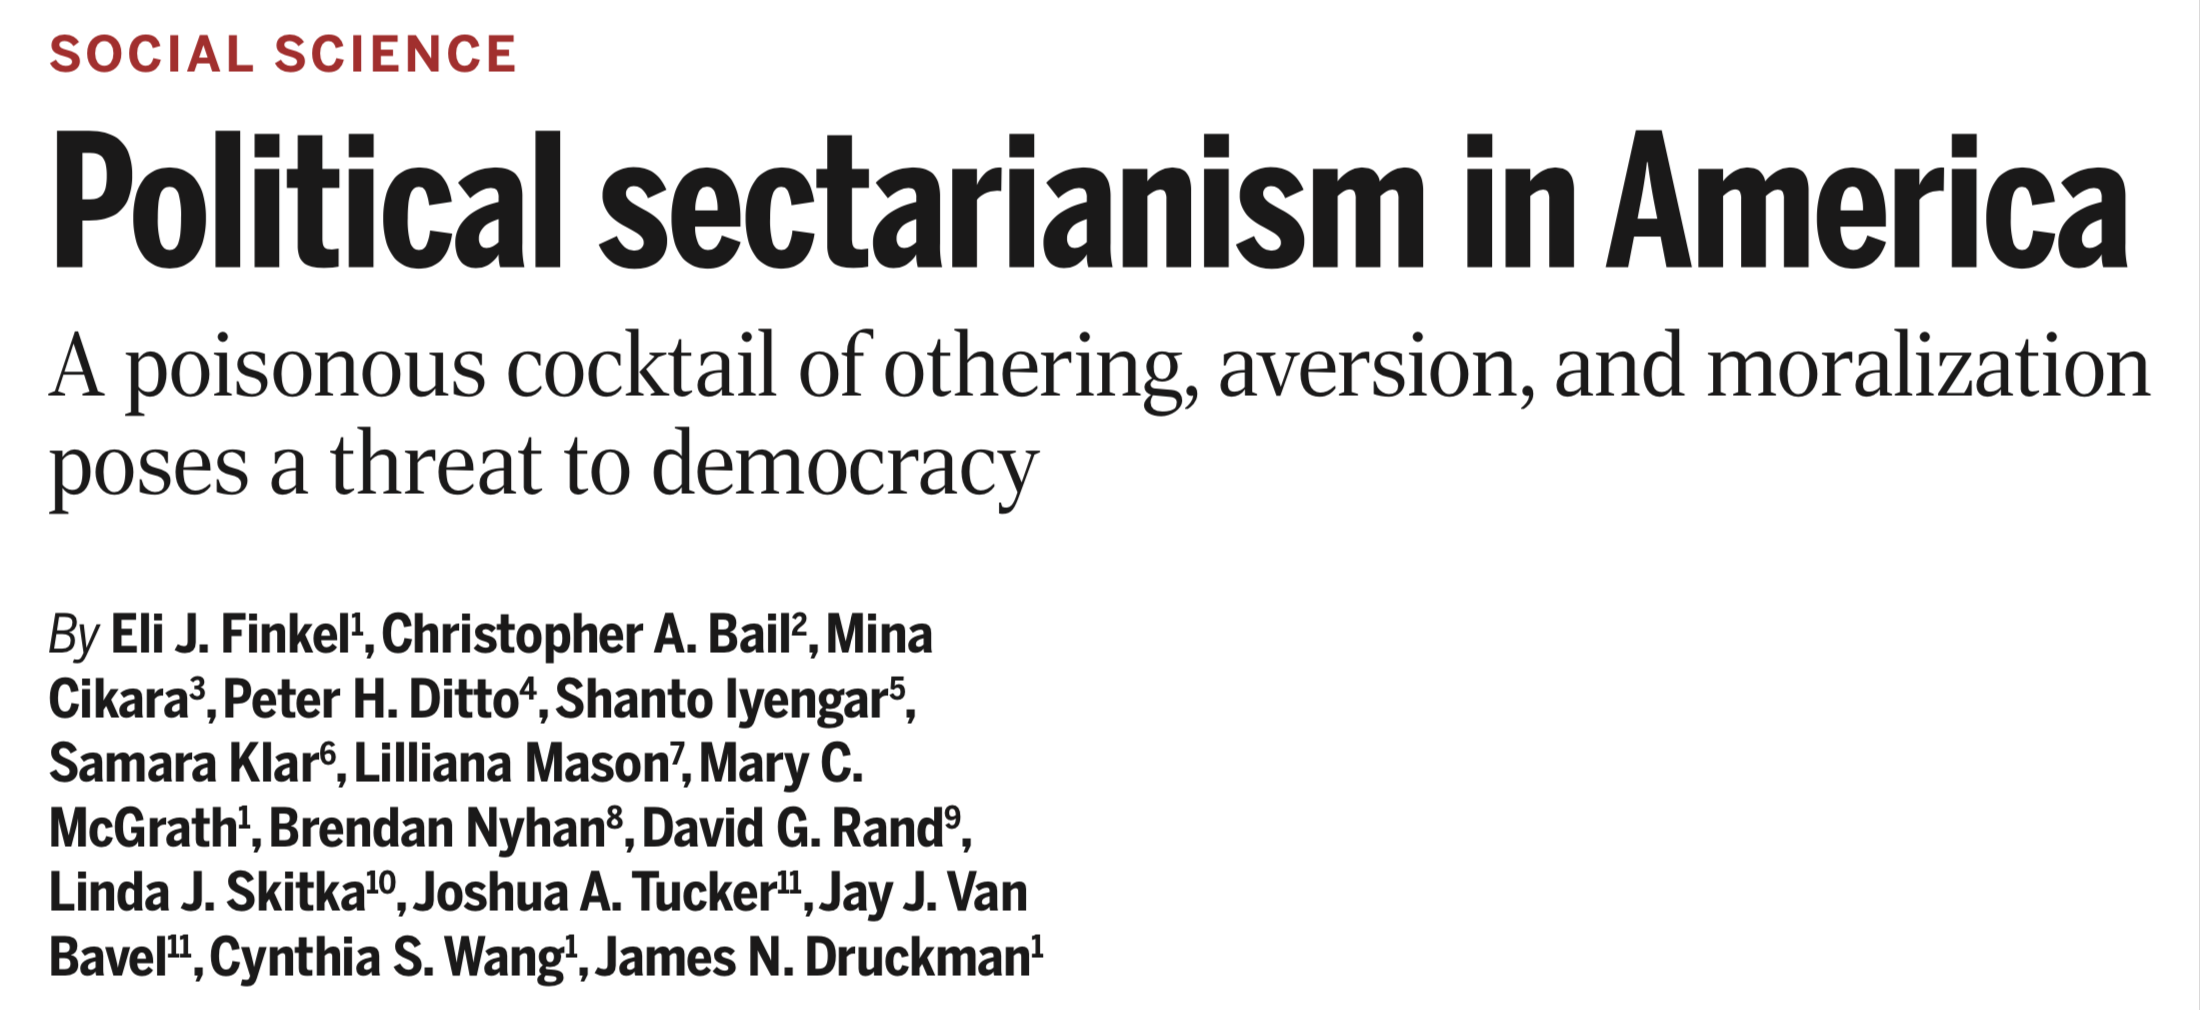
\includegraphics[width=0.95\textwidth]{figures/finkel_political_2020_title}
\end{center}

\end{frame}
%%%%%%%%%%%%%%%%%%%%%%%%%%%%%
\begin{frame}

\begin{center}
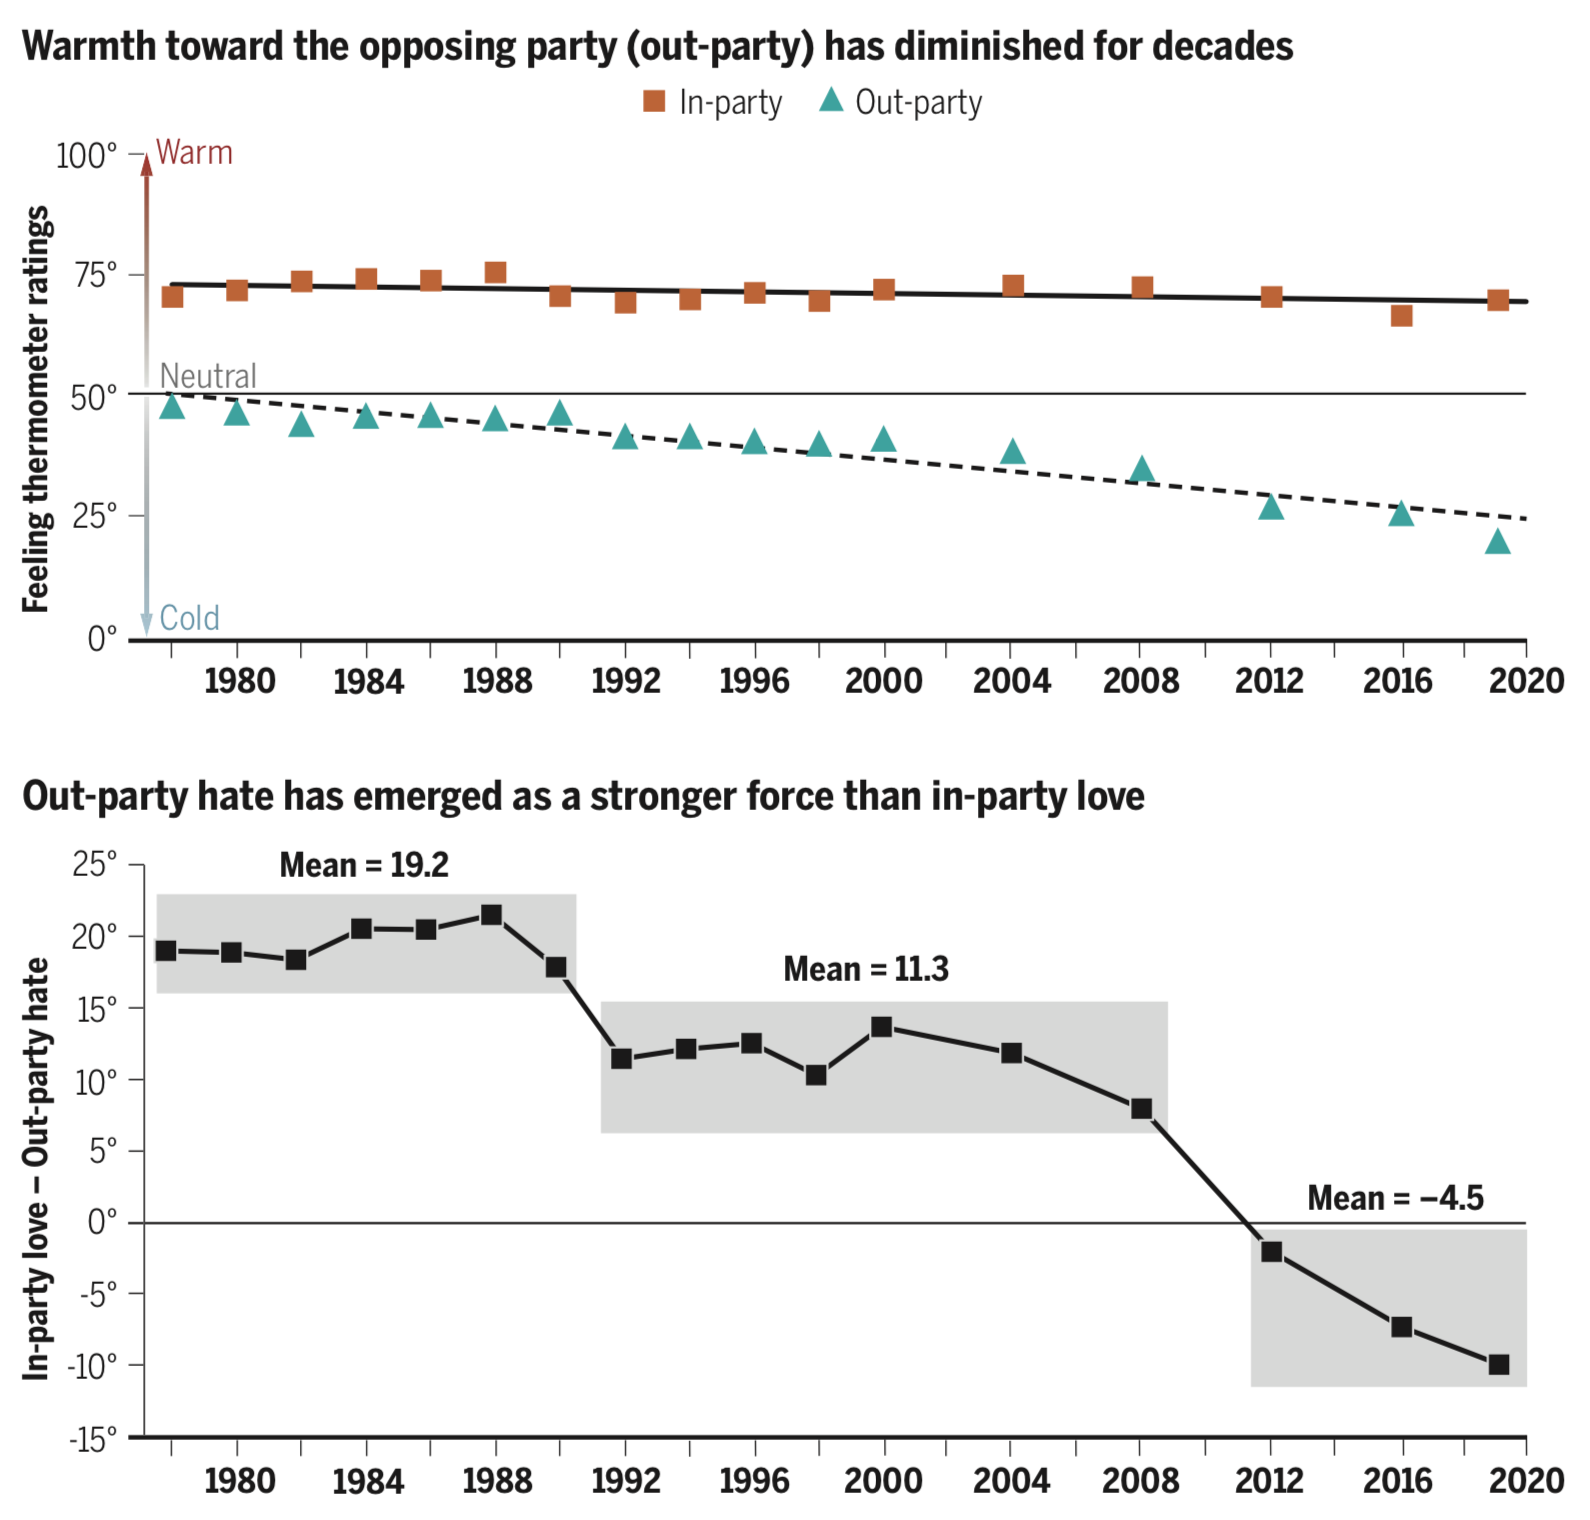
\includegraphics[height=0.95\textheight]{figures/finkel_political_2020_fig1}
\end{center}

\end{frame}
%%%%%%%%%%%%%%%%%%%%%%%%%
\begin{frame}

\begin{center}
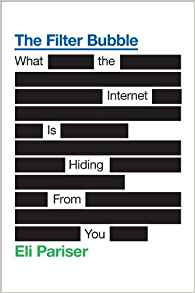
\includegraphics[height=0.85\textheight]{figures/pariser_filter_2011_cover}
\end{center}

Filter bubbles can be created by algorithms or choices of people

\note{
This study is not just about algorithms but people's choice
}

\end{frame}
%%%%%%%%%%%%%%%%%%%%%%%%%
\begin{frame}

\begin{center}
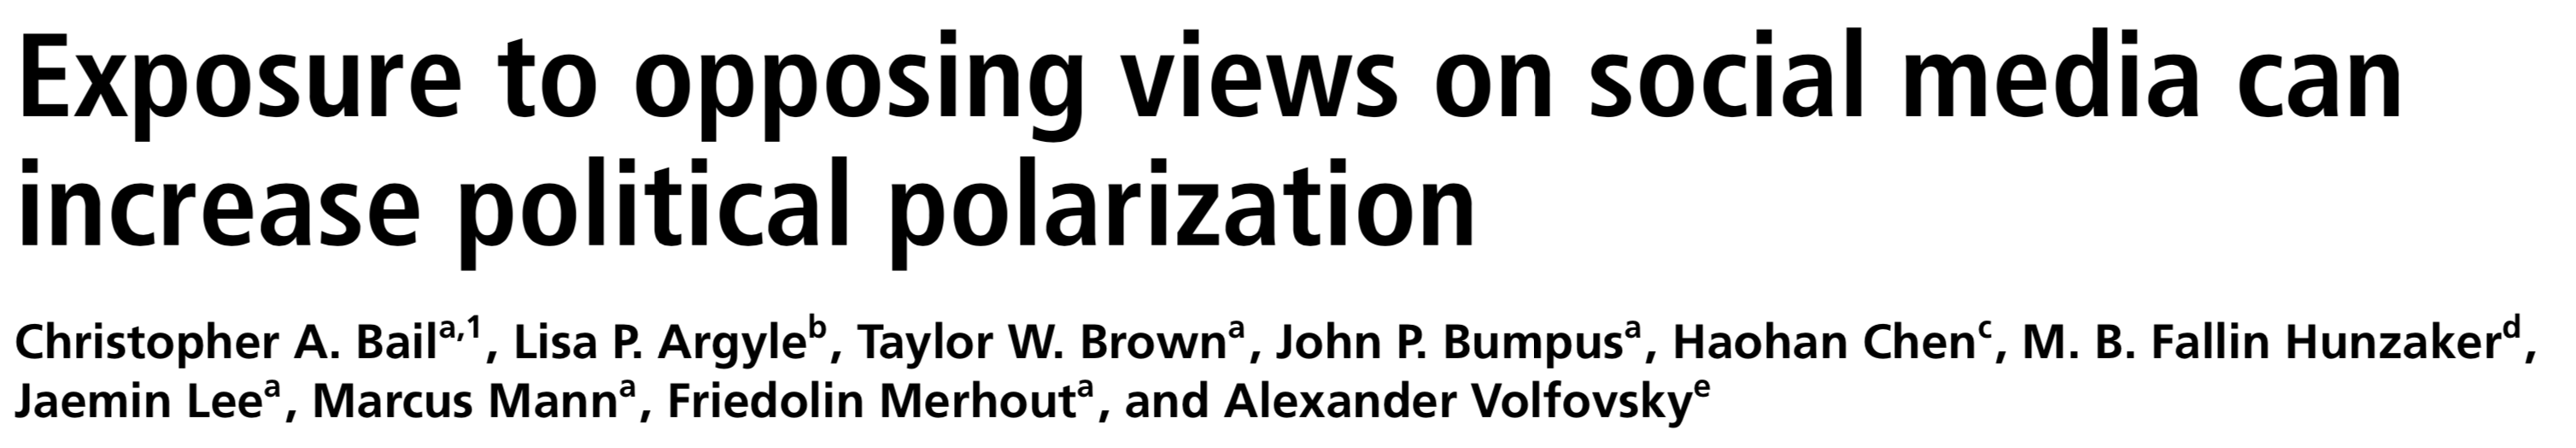
\includegraphics[width=\textwidth]{figures/bail_exposure_2018_title}
\end{center}

\end{frame}
%%%%%%%%%%%%%%%%%%%%%%
\begin{frame}

\begin{center}
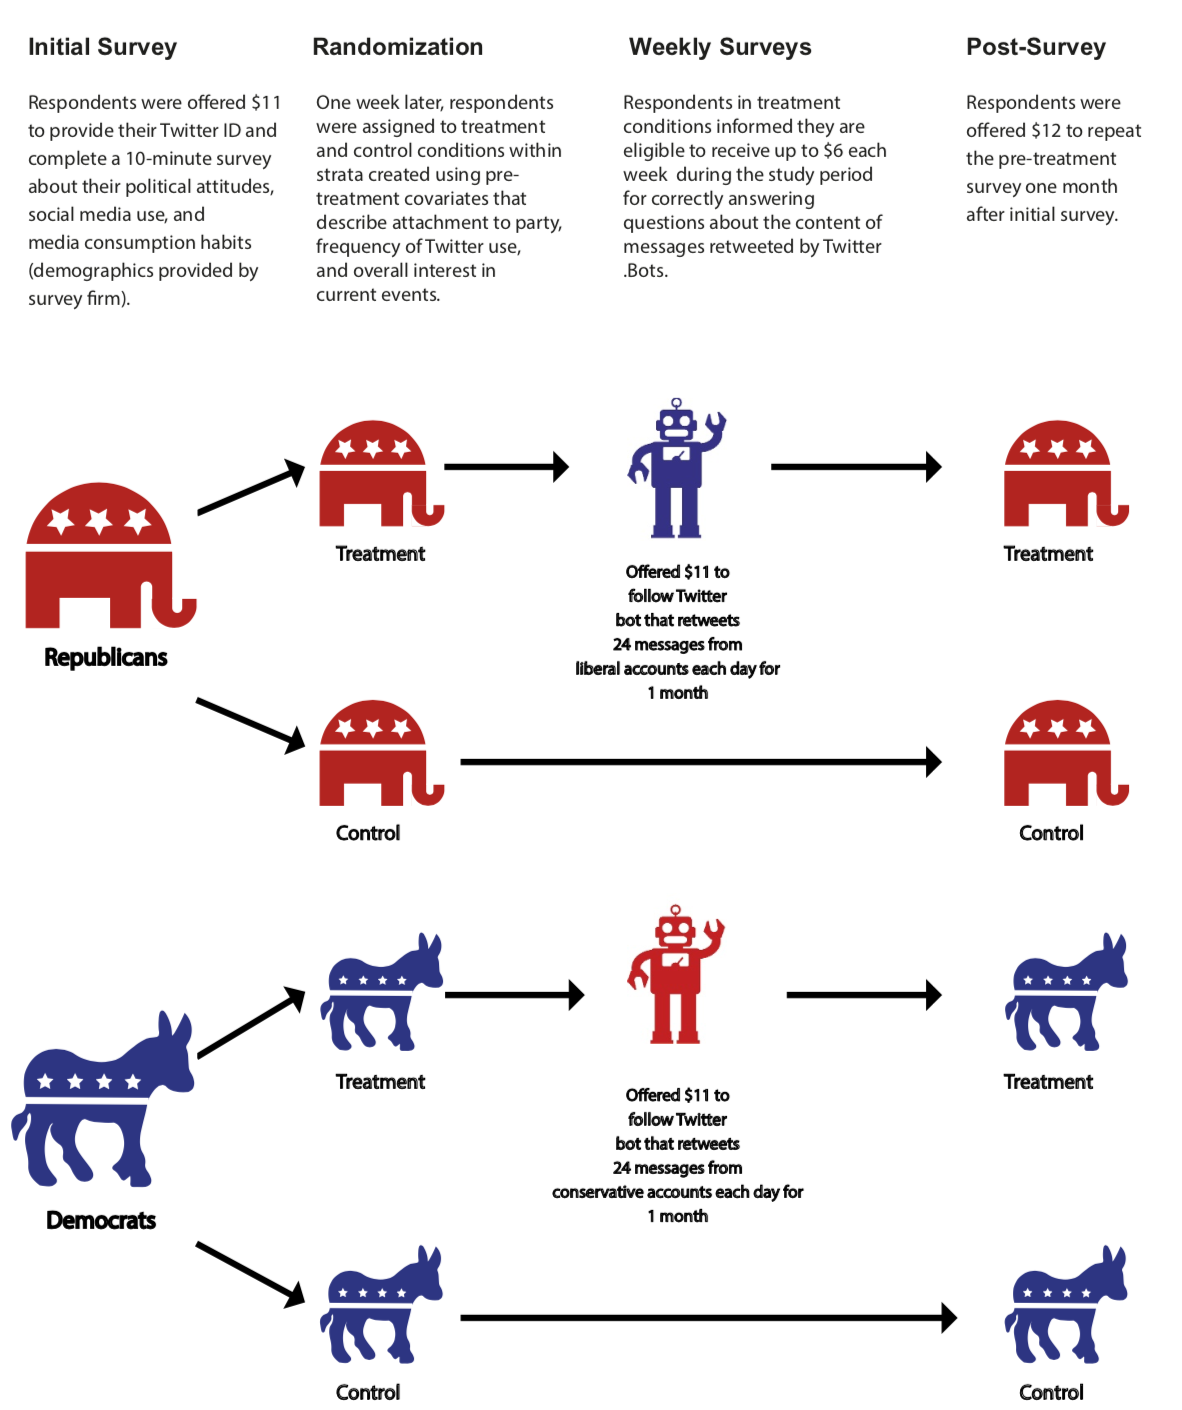
\includegraphics[width=0.4\textwidth]{figures/bail_exposure_2018_fig1}
\end{center}

\end{frame}
%%%%%%%%%%%%%%%%%%%%%%
\begin{frame}

Preregistered hypotheses
\begin{itemize}
\item disrupting selection exposure to partisan information will decrease political polarization \pause
\item exposure to opposing political views can increase political polarization \pause
\item backfire effects are more likely to occur among conservatives than liberals
\end{itemize}

\end{frame}
%%%%%%%%%%%%%%%%%%%%%%
\begin{frame}

\begin{center}
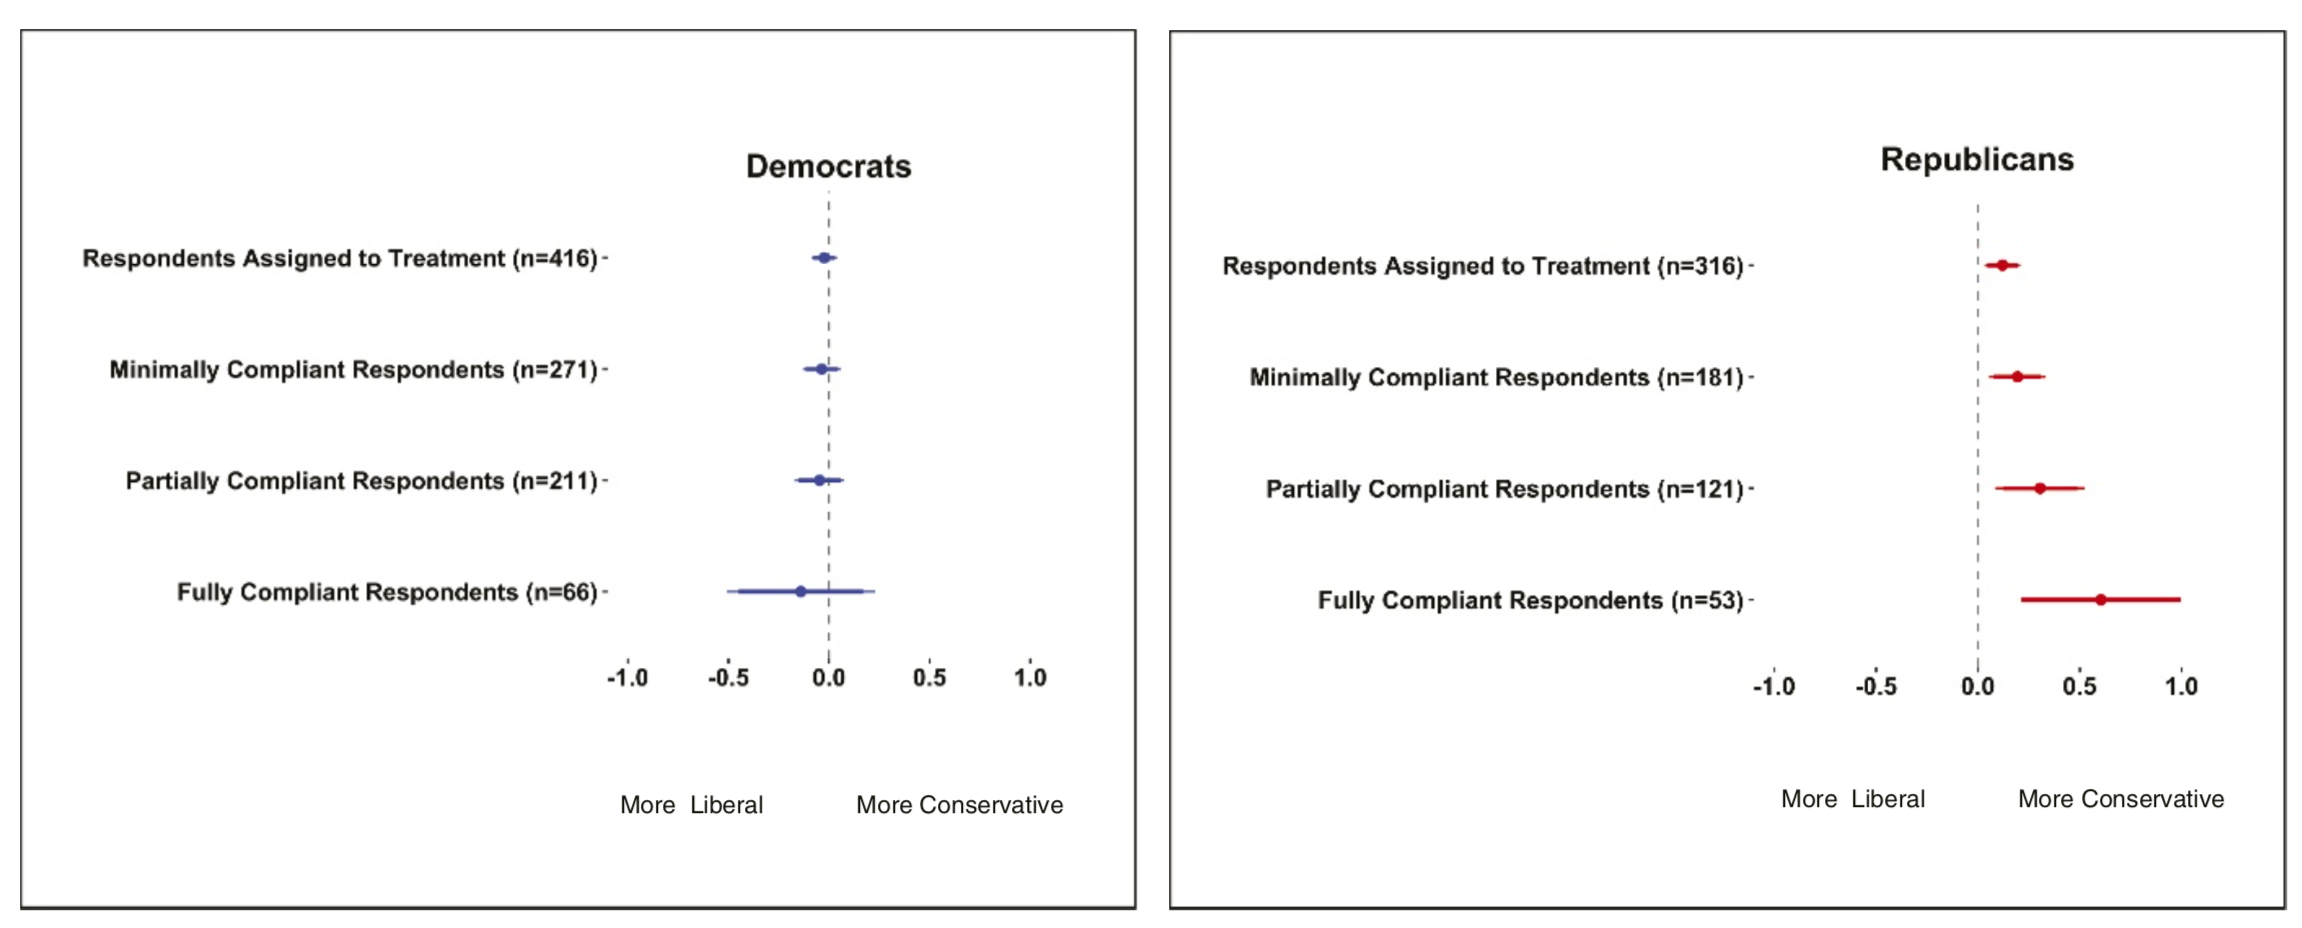
\includegraphics[width=0.8\textwidth]{figures/bail_exposure_2018_fig3}
\end{center}
\pause
\begin{itemize}
\item Democrats appear to become slightly more liberal, Republicans become more conservative \pause
\item Higher levels of compliance show larger effects\pause
\item unclear about exactly why this happened and whether it is specific to the way they constructed their bots
\end{itemize}

\end{frame}
%%%%%%%%%%%%%%%%%%%%%%
\begin{frame}

\begin{center}
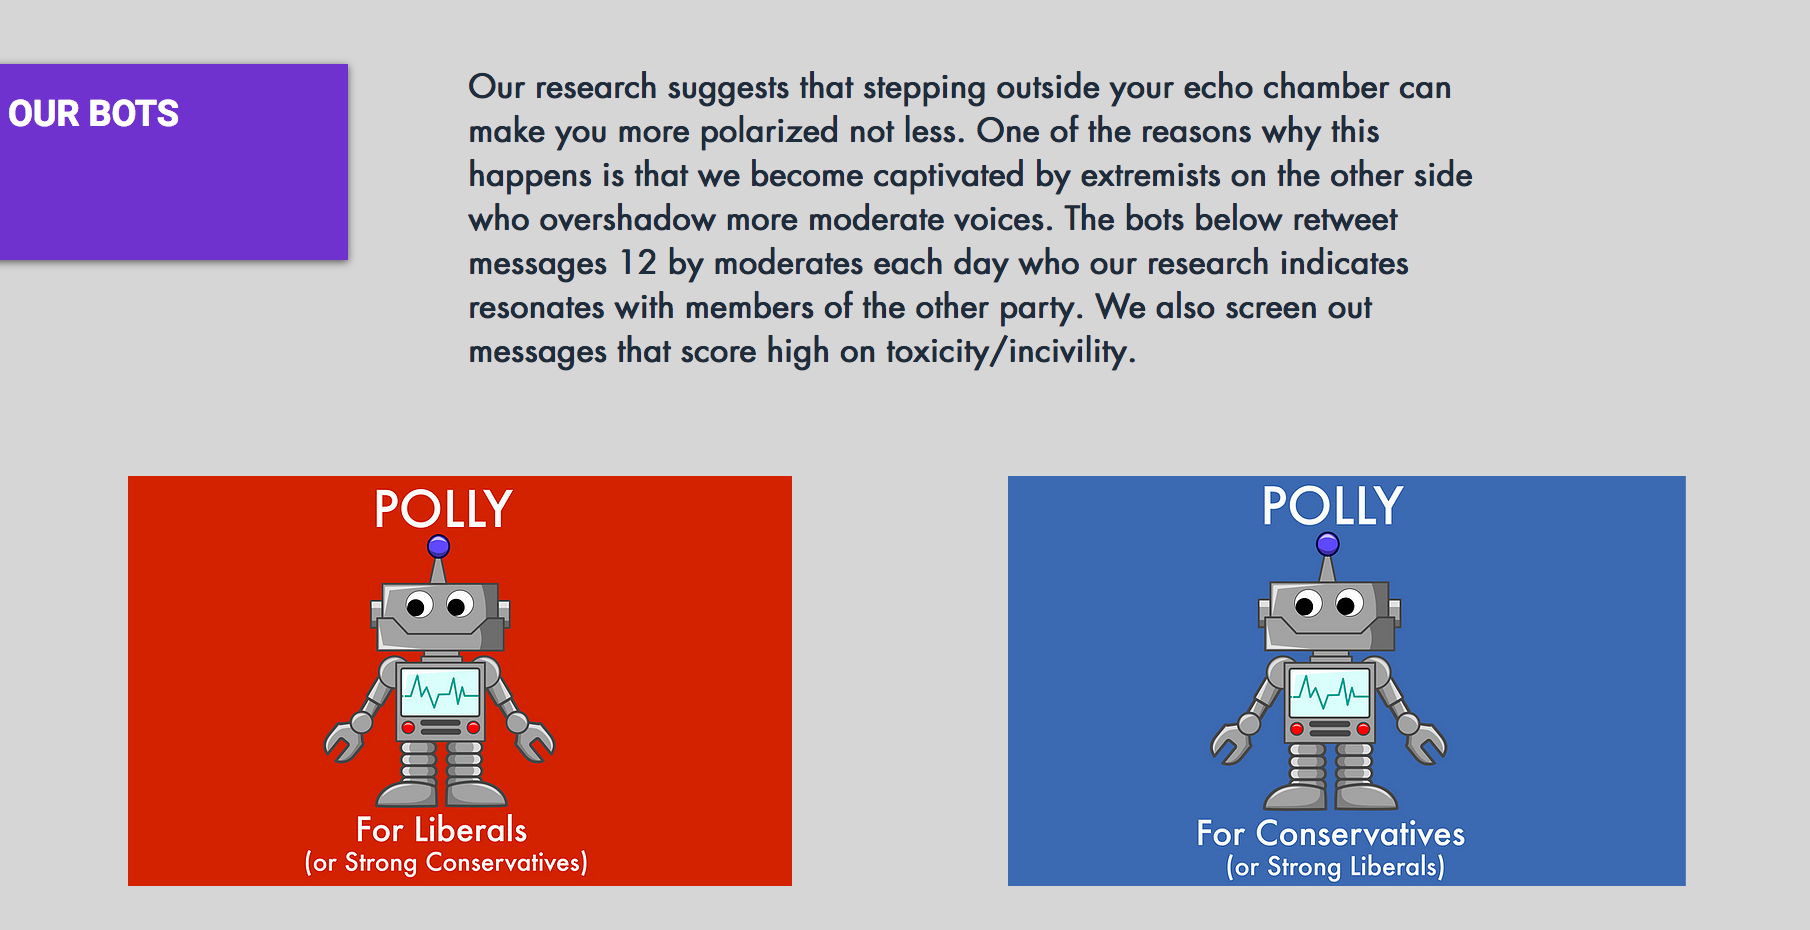
\includegraphics[width=\textwidth]{figures/polarization_lab_our_bots}
\end{center}

\vfill
\url{https://www.polarizationlab.com/our-bots}

\end{frame}
%%%%%%%%%%%%%%%%%%%%%%
\begin{frame}

\begin{center}
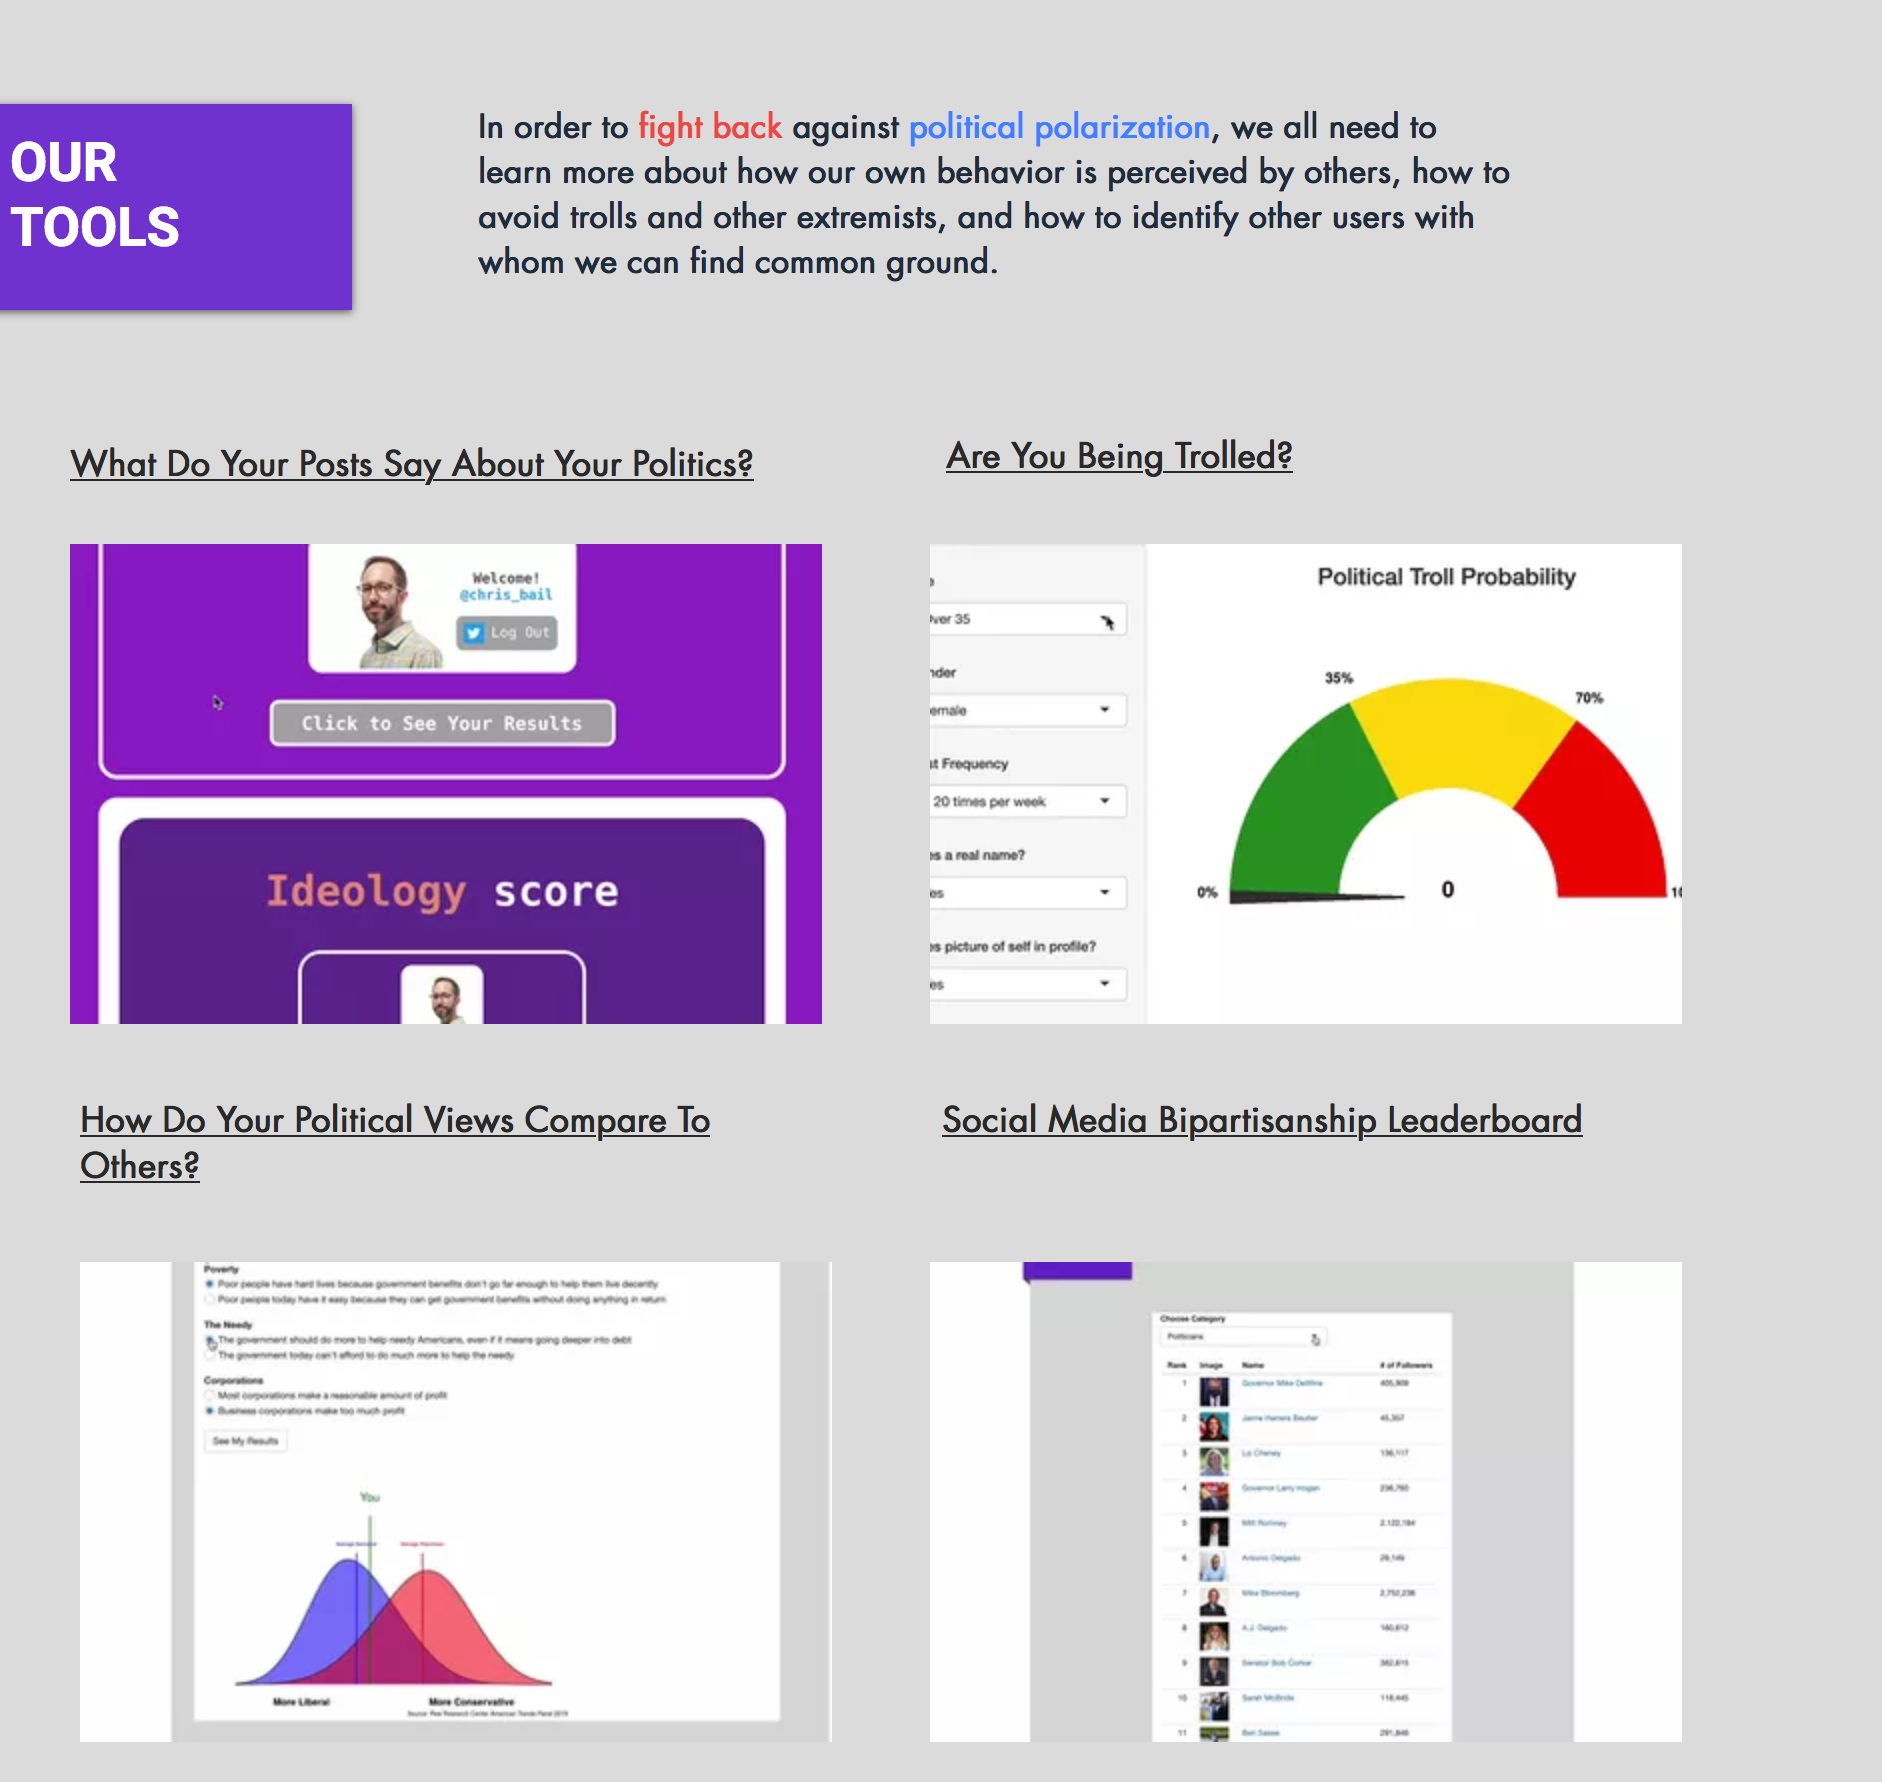
\includegraphics[width=0.5\textwidth]{figures/polarization_lab_our_tools}
\end{center}

\vfill
\url{https://www.polarizationlab.com/our-tools}

\end{frame}
%%%%%%%%%%%%%%%%%%%%%
\begin{frame}

\begin{center}
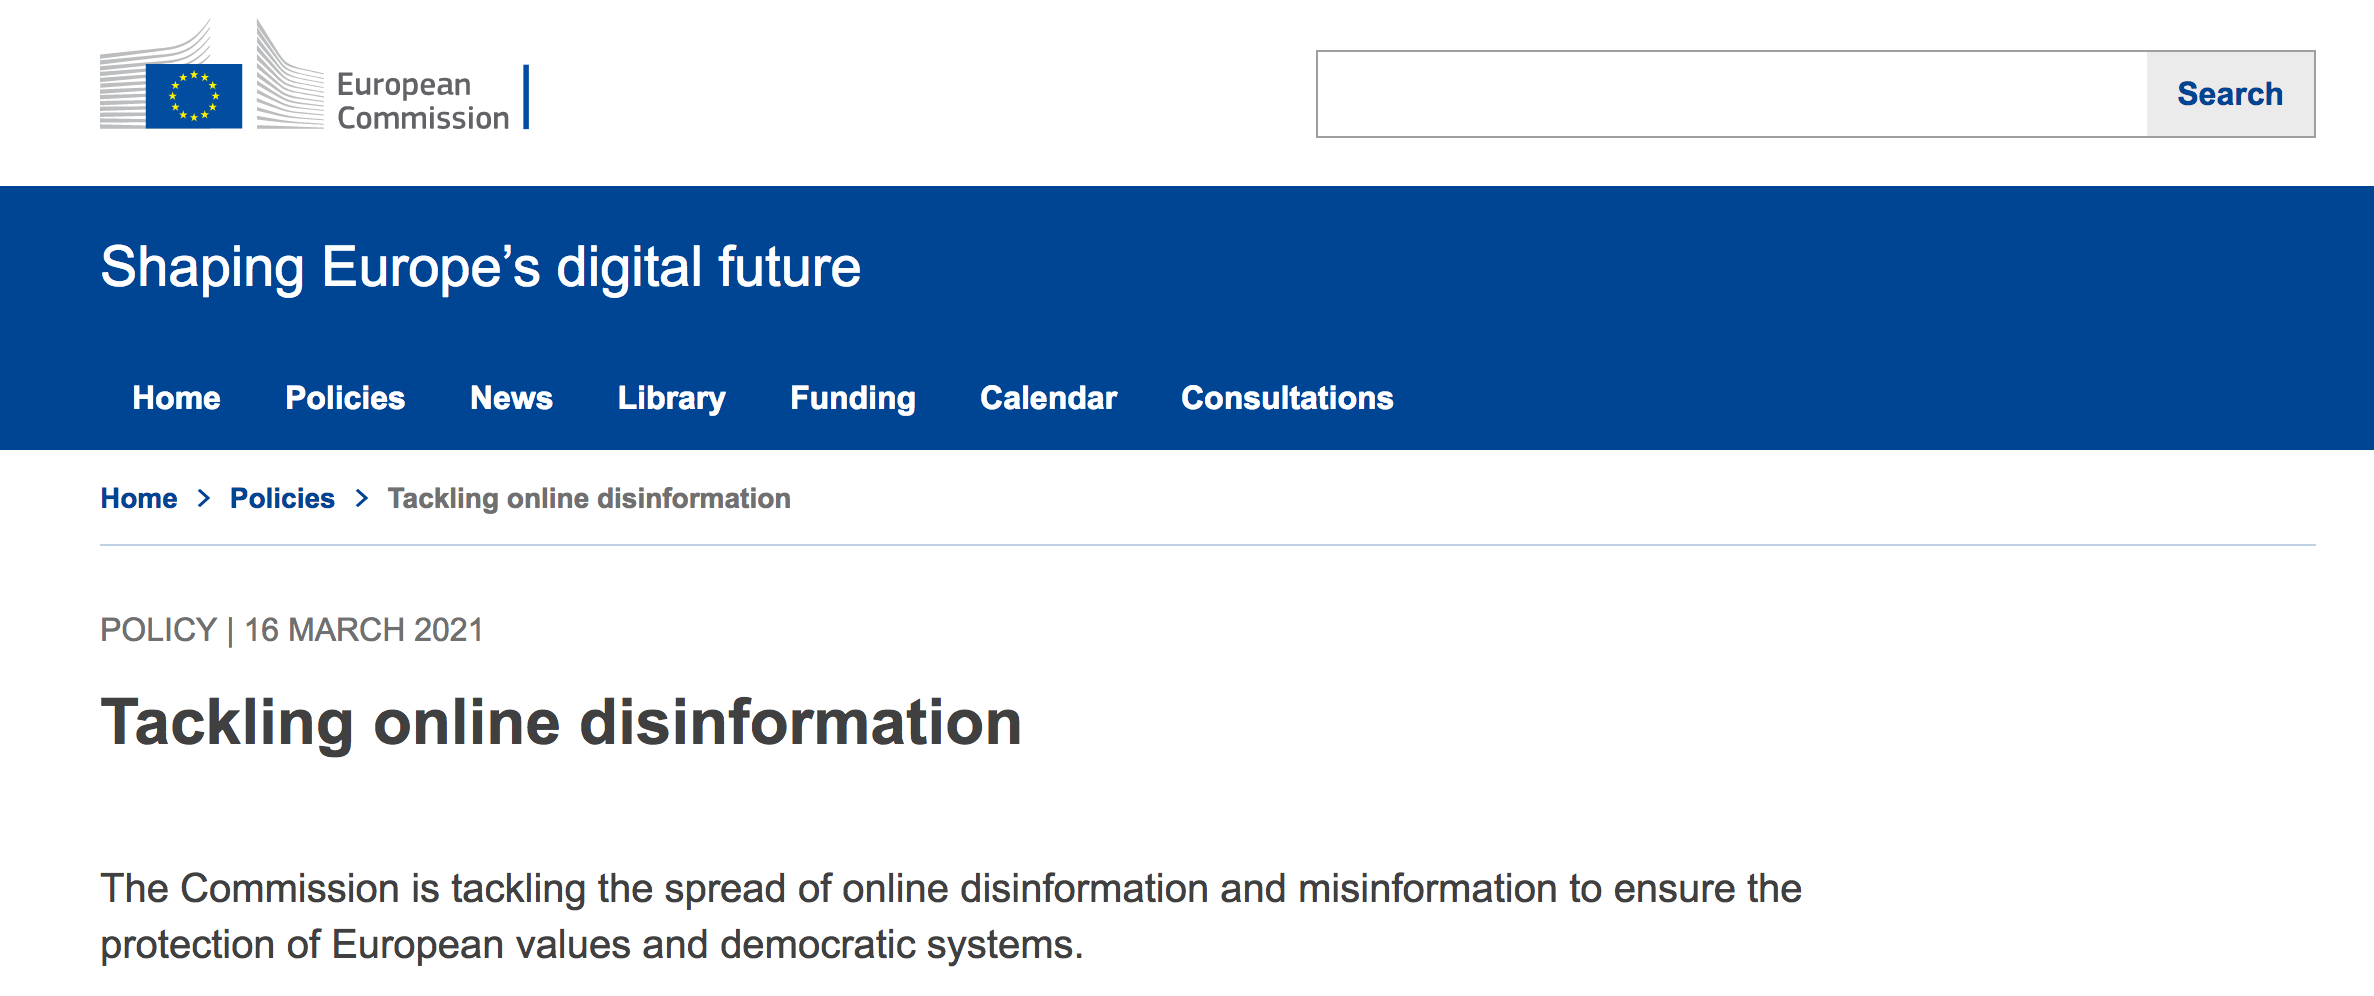
\includegraphics[width=\textwidth]{figures/eu_misinformation}
\end{center}

\url{https://digital-strategy.ec.europa.eu/en/policies/online-disinformation}

\end{frame}
%%%%%%%%%%%%%%%%%%%%%
\begin{frame}

3 common ways platforms deal with it
\begin{itemize}
\item derank \pause
\item remove content and people \pause
\item add warnings  \pause
\end{itemize}

\vfill
These approaches have different implications for free speech norms

\end{frame}
%%%%%%%%%%%%%%%%%%%%%
\begin{frame}

\setcounter{subfigure}{0}
\begin{figure}
  \centering
     \subfigure[Contextual warning]{
     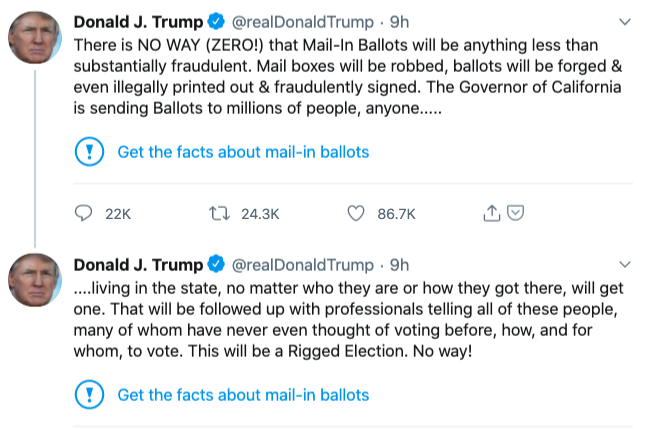
\includegraphics[width=0.45\textwidth]{figures/twitter_trump_warning}}
  \hspace{0in}
    \subfigure[Interstitial warning]{
    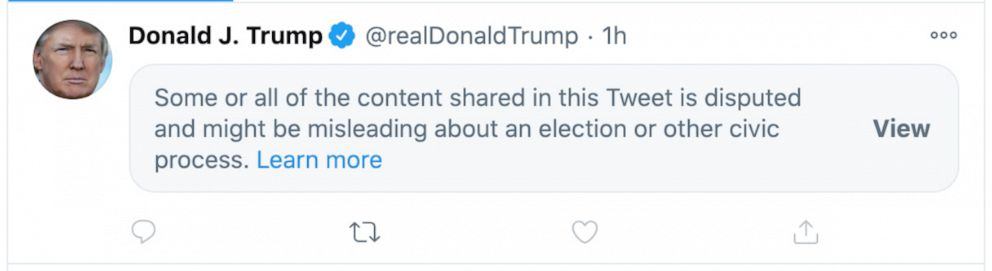
\includegraphics[width=0.45\textwidth]{figures/twitter_trump_interstitial}}
\end{figure}

What effects might these have?
\vfill
{\tiny \url{https://techcrunch.com/2020/05/26/twitter-trump-labels-fact-checking-tweet/}\\
\url{https://abcnews.go.com/Technology/twitter-facebook-slap-labels-trumps-misleading-election-posts/story?id=74020537}}

\end{frame}
%%%%%%%%%%%%%%%%%%%%%
\begin{frame}

\begin{center}
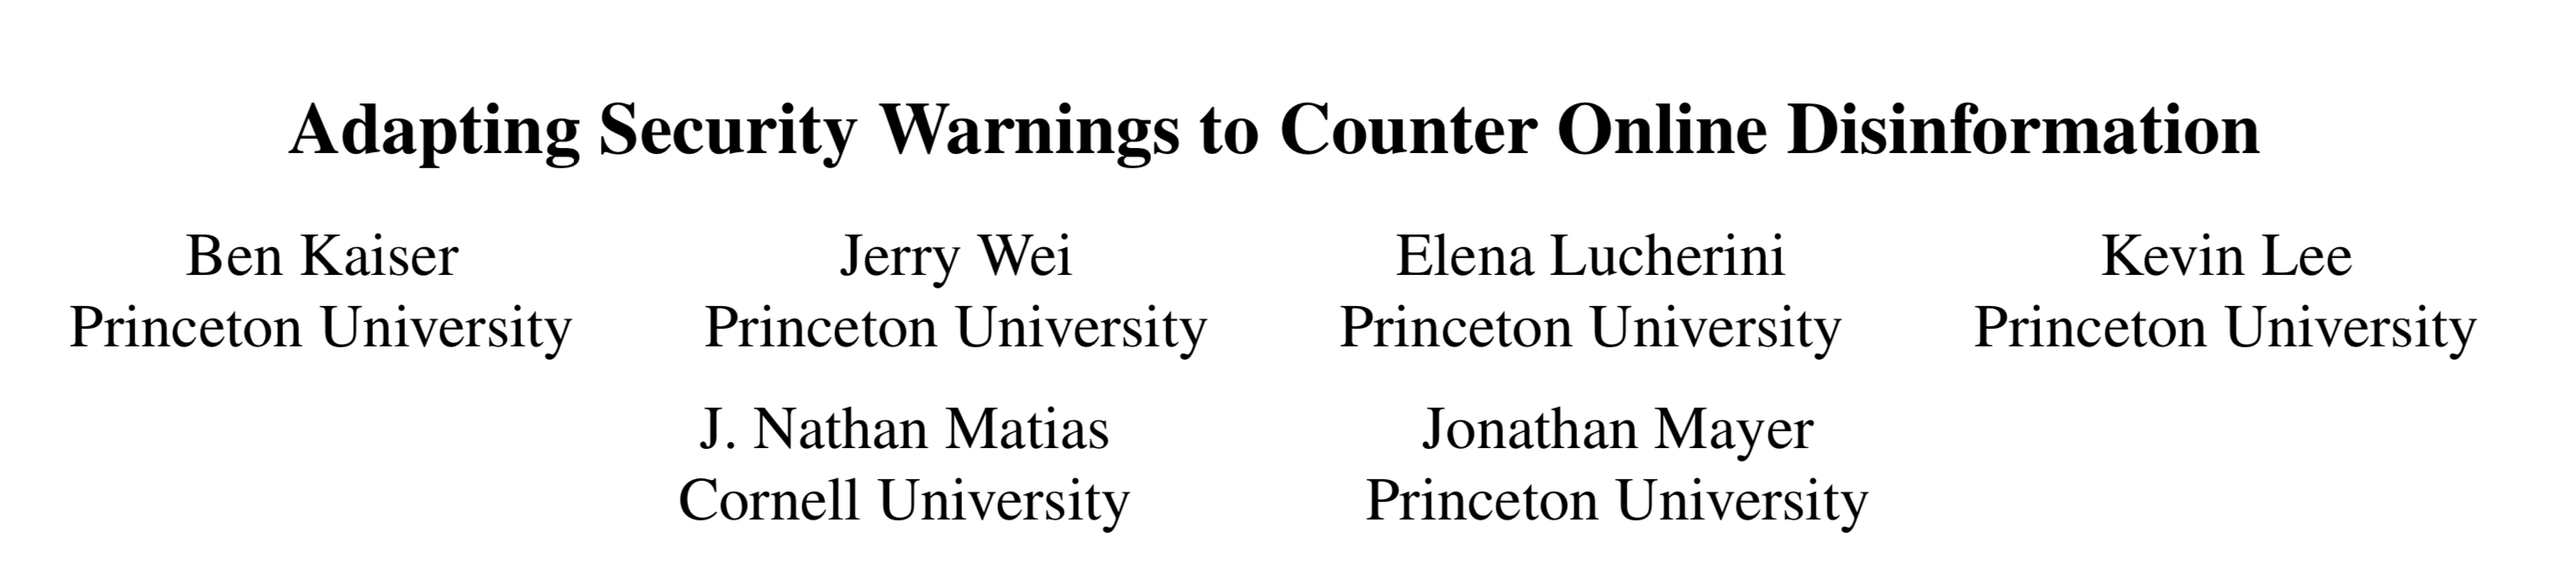
\includegraphics[width=\textwidth]{figures/kaiser_adapting_2020_title}
\end{center}

\begin{itemize}
\item 2 studies: 1 lab study with Princeton students, 1 online study on Mechanical Turk workers \pause
\item no cooperation from any social media platform \pause
\item does not address the challenge of deciding what is misinformation
\end{itemize}

\end{frame}
%%%%%%%%%%%%%%%%%%%%%
\begin{frame}

Study 1: Lab study of Princeton students

\setcounter{subfigure}{0}
\begin{figure}
  \centering
     \subfigure[Contextual warning]{
     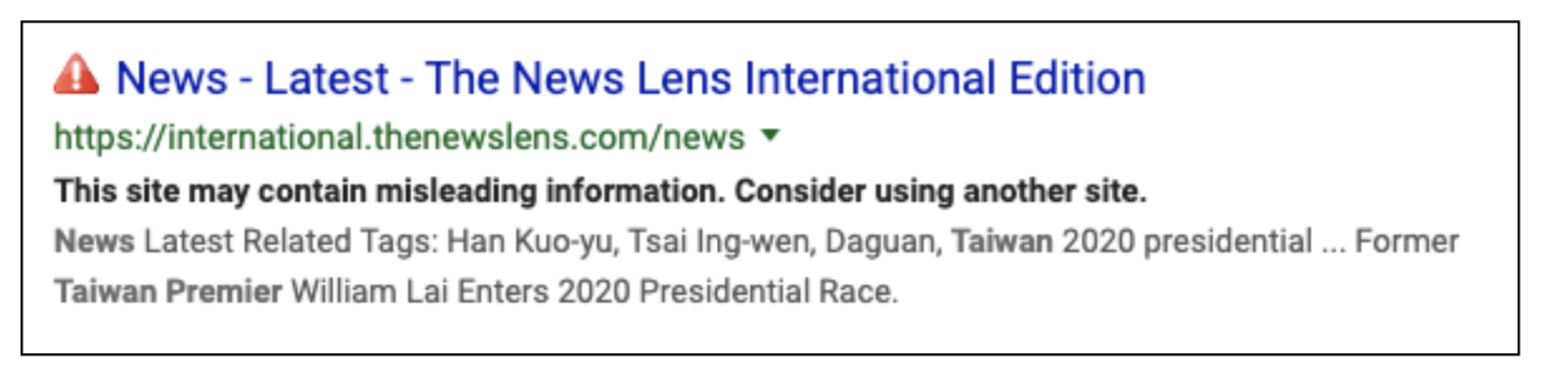
\includegraphics[width=0.45\textwidth]{figures/kaiser_adapting_2020_fig1}}
  \hspace{0in}
    \subfigure[Interstitial warning]{
    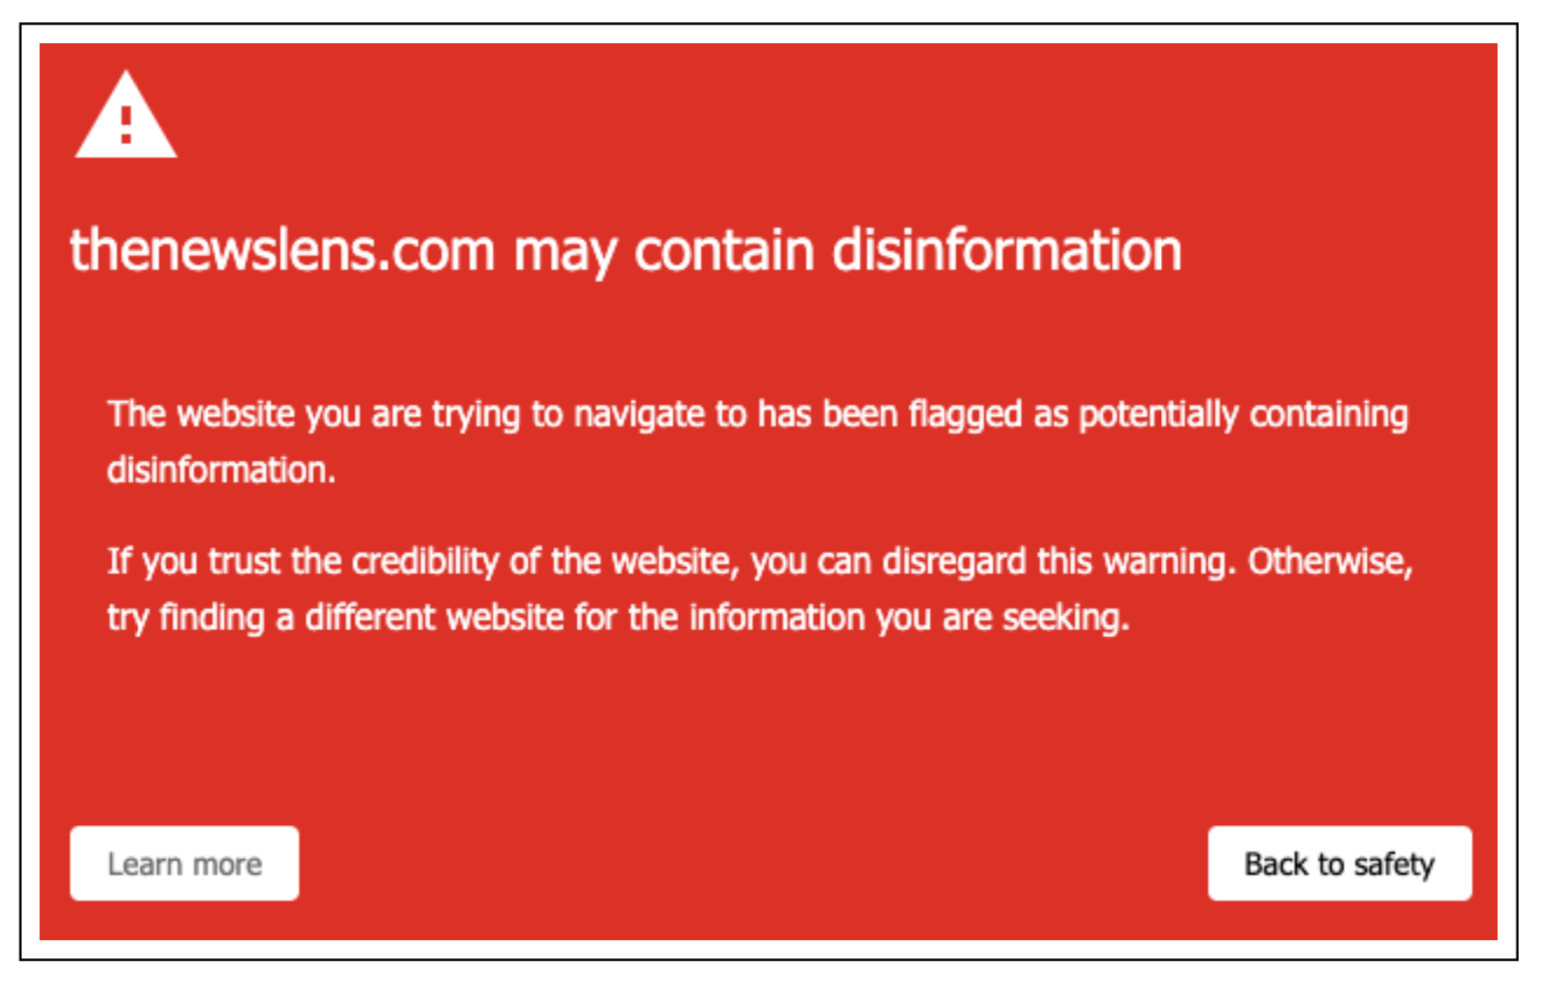
\includegraphics[width=0.45\textwidth]{figures/kaiser_adapting_2020_fig2}}
\end{figure}


\end{frame}
%%%%%%%%%%%%%%%%%%%%%
\begin{frame}

Study 1: Lab study of Princeton students

\setcounter{subfigure}{0}
\begin{figure}
  \centering
     \subfigure[Contextual warning]{
     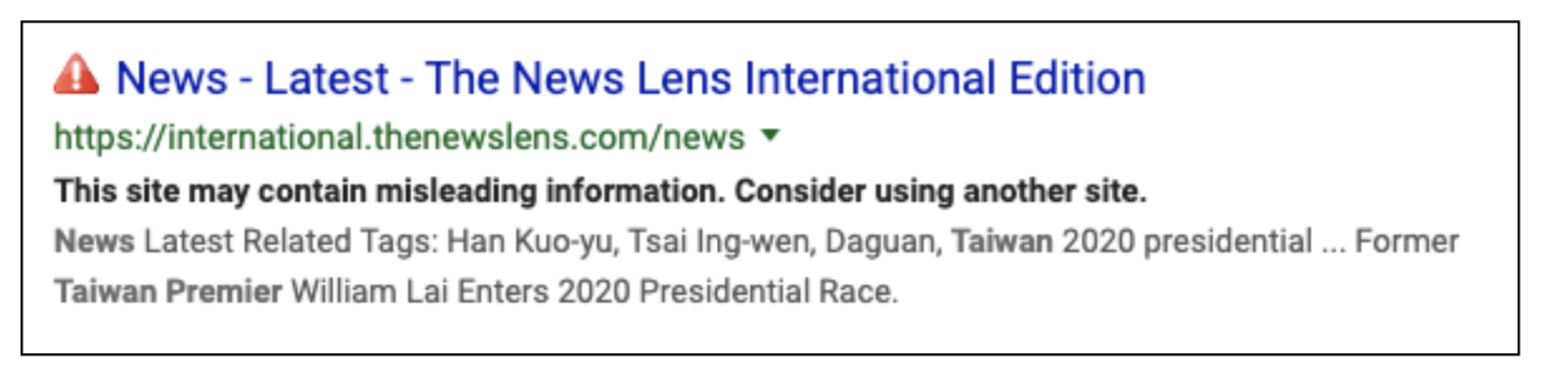
\includegraphics[width=0.45\textwidth]{figures/kaiser_adapting_2020_fig1}}
  \hspace{0in}
    \subfigure[Interstitial warning]{
    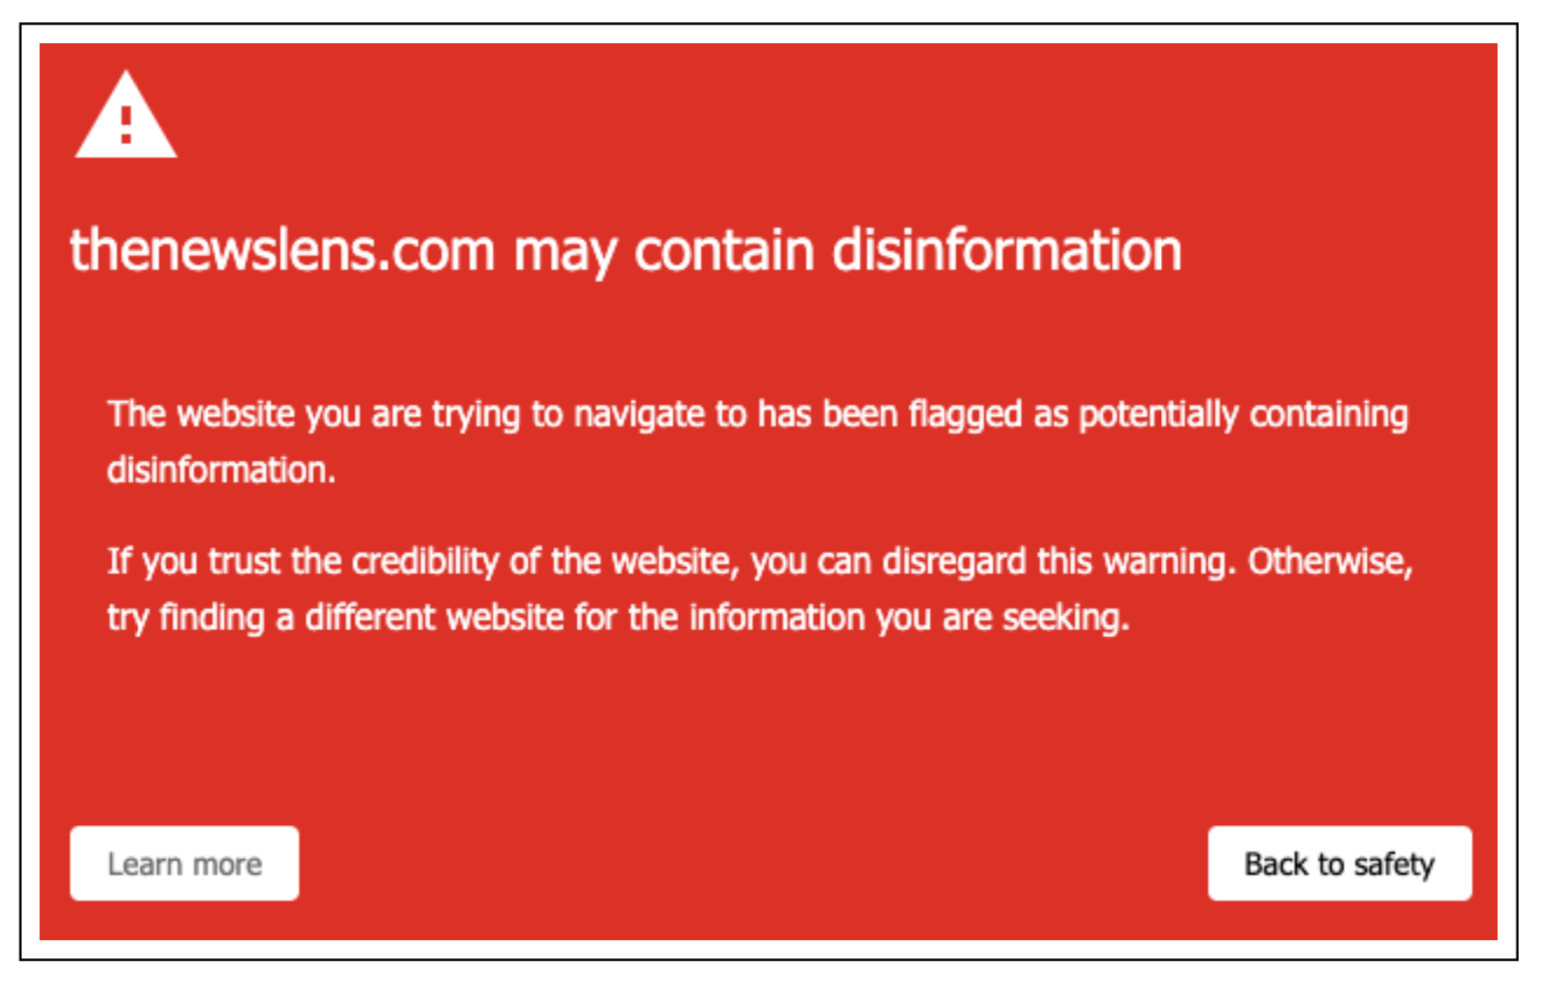
\includegraphics[width=0.45\textwidth]{figures/kaiser_adapting_2020_fig2}}
\end{figure}

\vfill
Quantitative metrics:
\begin{itemize}
\item Clickthrough rate (dismiss warning and proceed)
\item Alternative visit rate (proportion that visit alternative site as desired)
\end{itemize}

\end{frame}
%%%%%%%%%%%%%%%%%%%%%
\begin{frame}

\begin{center}
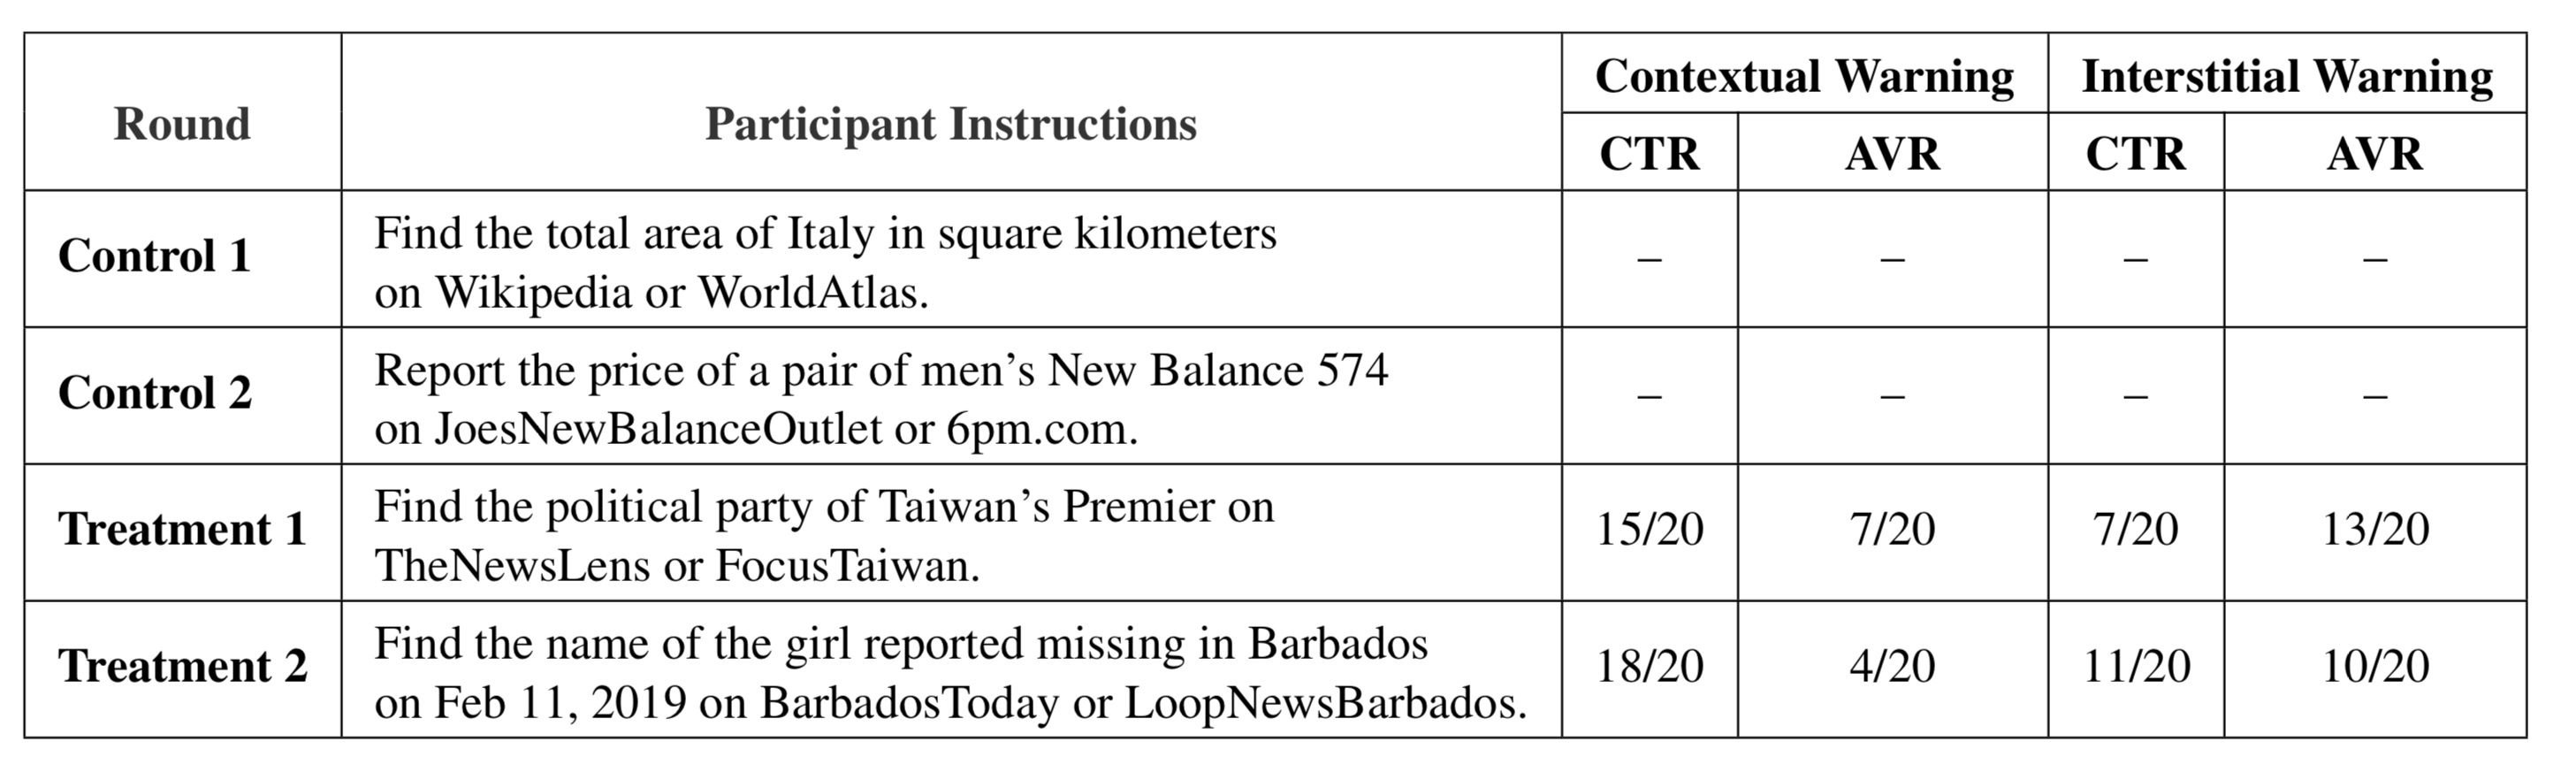
\includegraphics[width=\textwidth]{figures/kaiser_adapting_2020_tab1}
\end{center}

\begin{itemize}
\item Interstitial warning works better by both metrics (cllickthrough rate and alternative visit rate)
\end{itemize}

\end{frame}
%%%%%%%%%%%%%%%%%%%%%
\begin{frame}

Study 2: Workers on Amazon Mechanical Turk. Find the ``best'' interstitial warning.

\setcounter{subfigure}{0}
\begin{figure}
  \centering
     \subfigure[Harm]{
     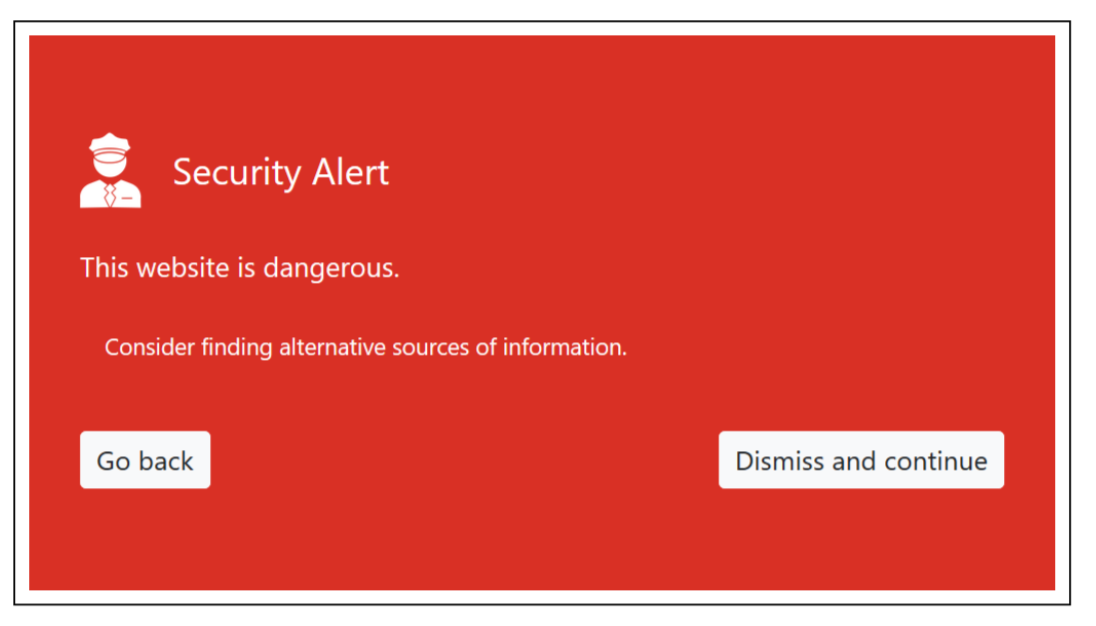
\includegraphics[width=0.45\textwidth]{figures/kaiser_adapting_2020_fig3b}}
  \hspace{0in}
    \subfigure[Informative]{
    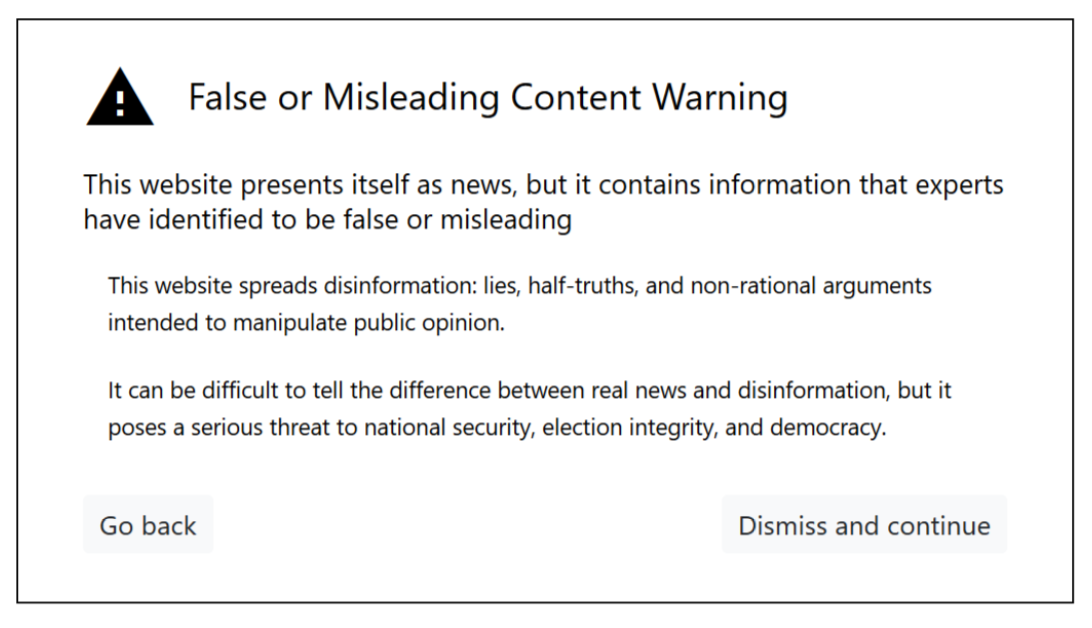
\includegraphics[width=0.45\textwidth]{figures/kaiser_adapting_2020_fig3a}}
\end{figure}
\end{frame}
%%%%%%%%%%%%%%%%%%%%%
\begin{frame}

\begin{center}
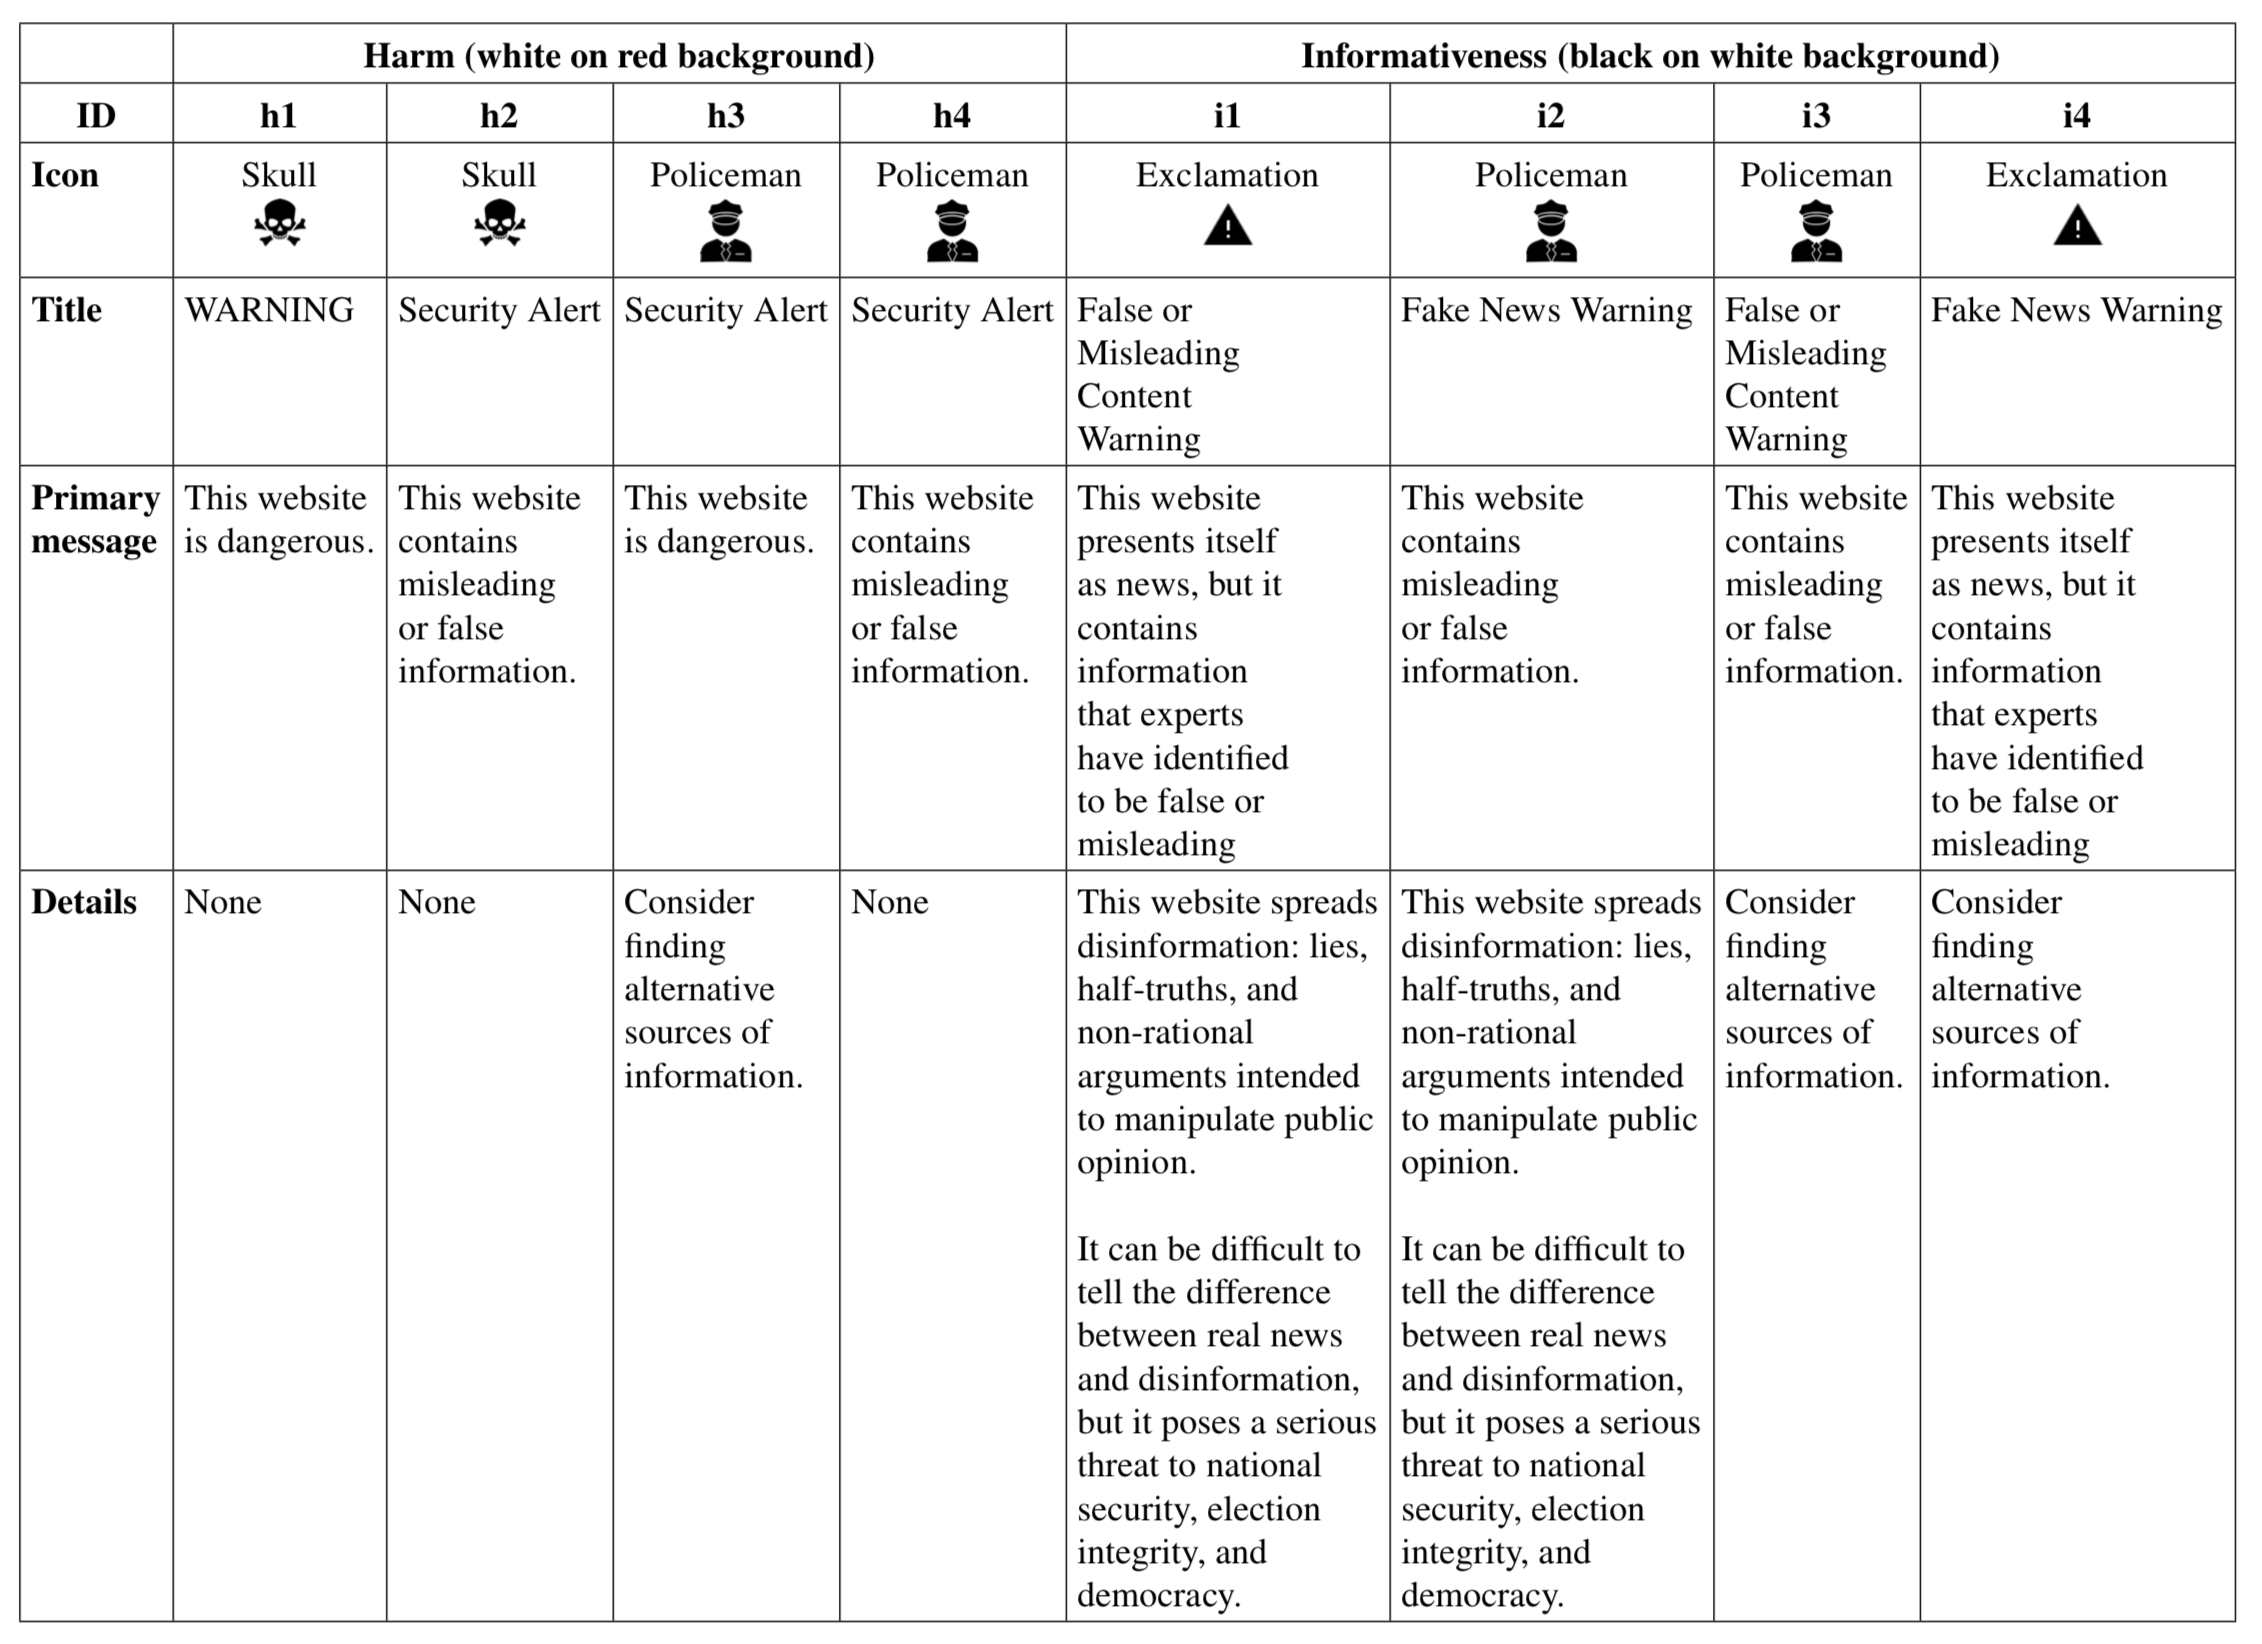
\includegraphics[width=0.6\textwidth]{figures/kaiser_adapting_2020_tab2}
\end{center}

Quantitative metrics:
\begin{itemize}
\item Clickthrough rate (dismiss warning and proceed)
\item Alternative visit rate (proportion that visit alternative site as desired)
\item Information score (based on survey)
\item Harm score (based on survey)
\end{itemize}

\end{frame}
%%%%%%%%%%%%%%%%%%%%%
\begin{frame}

\begin{center}
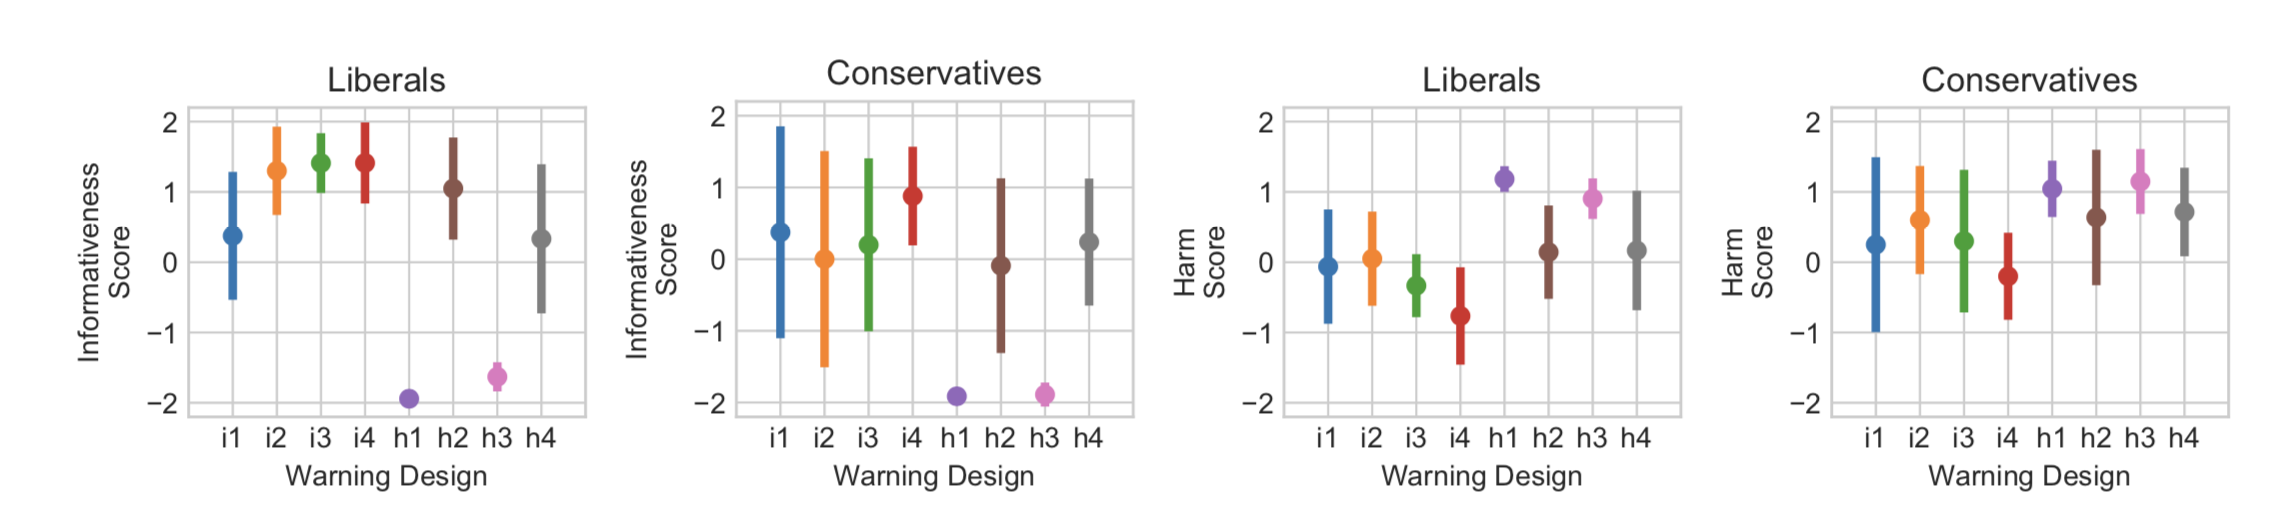
\includegraphics[width=\textwidth]{figures/kaiser_adapting_2020_fig6}
\end{center}

\begin{itemize}
\item With a few exceptions, not big differences between warnings, but small differences at scale can matter. \pause
\item Not big differences between liberals and conservatives, but small differences at scale can matter. \pause
\item If these were to be deployed, you would want to understand differences for many different subgroups.
\end{itemize}

\end{frame}
%%%%%%%%%%%%%%%%%%%%%
\begin{frame}

\begin{center}
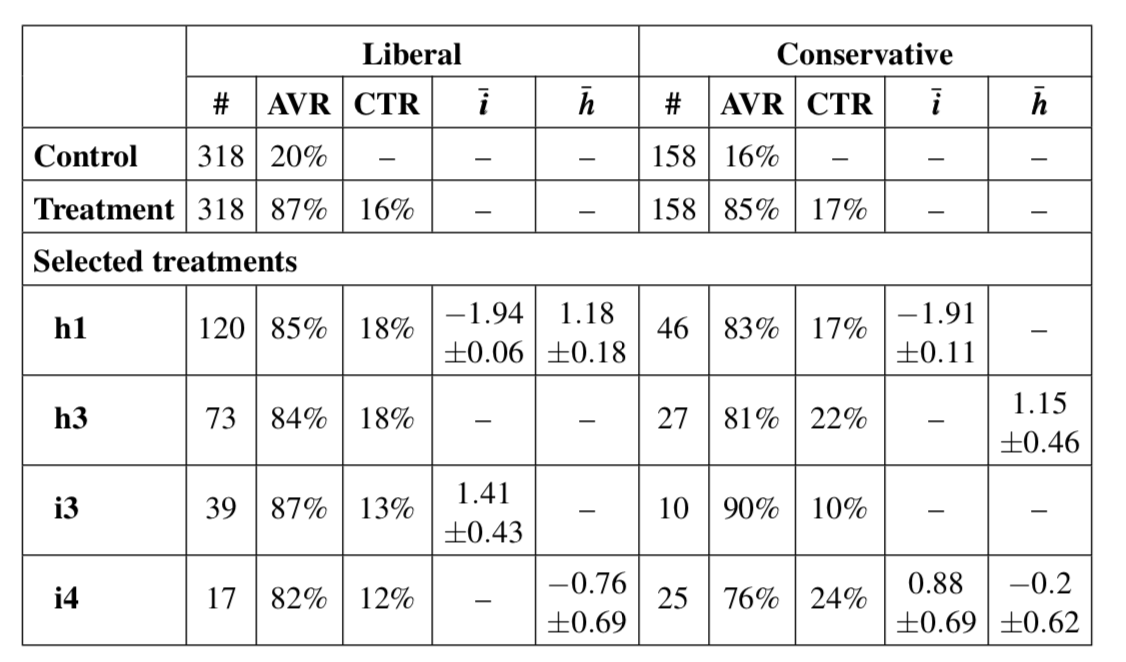
\includegraphics[width=0.7\textwidth]{figures/kaiser_adapting_2020_tab4}
\end{center}

\begin{itemize}
\item With a few exceptions, not big differences between warnings, but small differences at scale can matter. \pause
\item Sample sizes are really small here so we should have caution
\end{itemize}

\end{frame}
%%%%%%%%%%%%%%%%%%%%%
\begin{frame}

\setcounter{subfigure}{0}
\begin{figure}
  \centering
     \subfigure[Contextual warning]{
     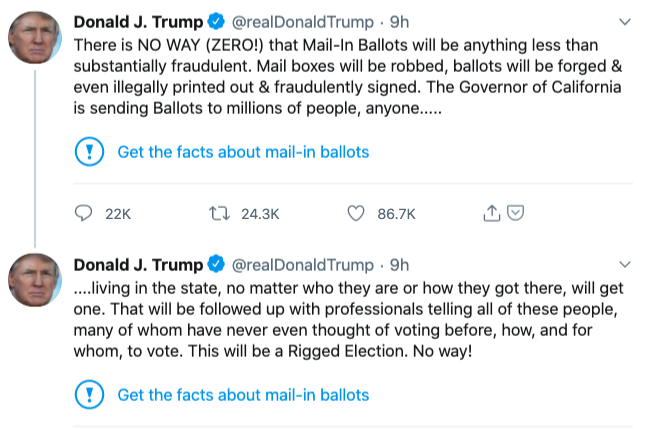
\includegraphics[width=0.45\textwidth]{figures/twitter_trump_warning}}
  \hspace{0in}
    \subfigure[Interstitial warning]{
    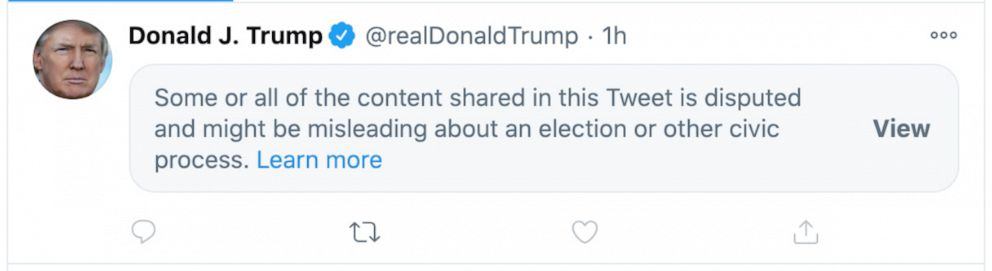
\includegraphics[width=0.45\textwidth]{figures/twitter_trump_interstitial}}
\end{figure}

What effects might these have?
\vfill
{\tiny \url{https://techcrunch.com/2020/05/26/twitter-trump-labels-fact-checking-tweet/}\\
\url{https://abcnews.go.com/Technology/twitter-facebook-slap-labels-trumps-misleading-election-posts/story?id=74020537}}

\end{frame}
%%%%%%%%%%%%%%%%%%%%%
\begin{frame}

Conclusions:
\begin{itemize}
\item Interventions to change social media could be either structural changes or tweaks \pause
\item We have solid evidence that tweaks don't always have the intended effects (Bail et al.) \pause
\item We have solid evidence that the relative effectiveness of tweaks is hard to anticipate (Kaiser et al.) \pause
\item It will be even hard to anticipate all the effects of structural changes, but that does not have to be a recipe for inaction
\end{itemize}

\end{frame}
%%%%%%%%%%%%%%%%%%%%%
\begin{frame}

Social media:
\begin{itemize}
\item Social media and individuals
\item Social media and society
\item Social media and social ads
\item Fixing social media
\end{itemize}

\end{frame}
%%%%%%%%%%%%%%%%%%%%%
\begin{frame}

Class 22: Network scale-up method to study groups most at-risk for HIV 
\begin{itemize}
\item Feehan, D.M. and Salganik, M.J. (2016). Generalizing the Network Scale-up Method: A New Estimator for the Size of Hidden Populations. \textit{Sociological Methodology}.
\item Feehan, D.M. et al. (2016). Quality vs. Quantity: A survey experiment to improve the network scale-up method. \textit{American Journal of Epidemiology}. 
\end{itemize}

\end{frame}
%%%%%%%%%%%%%%%%%%%%%


\end{document}
